% presentation_v2_eng.tex
% Beamer slides for the oral presentation — Perceiver Project (V2 English)
% Compile with: pdflatex presentation_v2_eng.tex (x2 for TOC)

\documentclass[aspectratio=169,11pt]{beamer}

% ── Theme and Colors ─────────────────────────────────────────────────────────
\usetheme{Madrid}
\usecolortheme{default}

\definecolor{UnifiBlue}{RGB}{0,82,147}
\definecolor{UnifiDark}{RGB}{33,37,41}
\definecolor{AccentOrange}{RGB}{230,126,34}
\definecolor{AccentGreen}{RGB}{39,174,96}
\definecolor{AccentRed}{RGB}{231,76,60}

% Apply colors to theme
\setbeamercolor{structure}{fg=UnifiBlue}
\setbeamercolor{title}{fg=white, bg=UnifiBlue}
\setbeamercolor{frametitle}{fg=white, bg=UnifiBlue}
\setbeamercolor{itemize item}{fg=UnifiBlue}
\setbeamercolor{itemize subitem}{fg=UnifiBlue!80}
\setbeamercolor{block title}{bg=UnifiBlue, fg=white}
\setbeamercolor{block body}{bg=UnifiBlue!10, fg=UnifiDark}
\setbeamercolor{block title alerted}{bg=AccentRed, fg=white}
\setbeamercolor{block body alerted}{bg=AccentRed!10, fg=UnifiDark}
\setbeamercolor{block title example}{bg=AccentGreen, fg=white}
\setbeamercolor{block body example}{bg=AccentGreen!10, fg=UnifiDark}
\setbeamercolor{alerted text}{fg=AccentOrange}

% Remove navigation symbols
\setbeamertemplate{navigation symbols}{}

% Footer format
\setbeamertemplate{footline}{%
  \leavevmode\hbox{%
    \begin{beamercolorbox}[wd=.42\paperwidth,ht=2.5ex,dp=1ex,center]{author in head/foot}%
      \usebeamerfont{author in head/foot}\scriptsize\insertshortauthor
    \end{beamercolorbox}%
    \begin{beamercolorbox}[wd=.40\paperwidth,ht=2.5ex,dp=1ex,center]{title in head/foot}%
      \usebeamerfont{title in head/foot}\scriptsize\insertshorttitle
    \end{beamercolorbox}%
    \begin{beamercolorbox}[wd=.18\paperwidth,ht=2.5ex,dp=1ex,right]{date in head/foot}%
      \usebeamerfont{date in head/foot}\scriptsize\insertframenumber{}/\inserttotalframenumber\hspace*{2ex}
    \end{beamercolorbox}%
  }%
}

% ── Packages ─────────────────────────────────────────────────────────────────
\usepackage[utf8]{inputenc}
\usepackage[T1]{fontenc}
\usepackage[english]{babel}
\usepackage{graphicx}
\usepackage{booktabs}
\usepackage{array}
\usepackage{amsmath,amssymb}
\usepackage{multirow}
\usepackage{tikz}
\usepackage{pgfplots}
\usepackage{hyperref}
\usepackage{fontawesome5}

\usetikzlibrary{arrows.meta,positioning,calc,fit,backgrounds,shapes.geometric,decorations.pathreplacing}
\pgfplotsset{compat=1.18}

% ── Shared style for inline bar charts (matches the matplotlib PNG charts) ────
\definecolor{ChartBlue}{HTML}{1F6BBD}
\definecolor{ChartNavy}{HTML}{123A6D}
\pgfplotsset{
  resultbar/.style={
    ybar,
    axis lines*=left,
    axis line style={gray!45, line width=0.5pt},
    ymajorgrids,
    grid style={gray!22, line width=0.5pt},
    tick style={draw=none},
    ylabel style={font=\small, color=gray!55!black},
    y tick label style={font=\scriptsize, color=gray!55!black},
    x tick label style={font=\scriptsize, color=ChartNavy},
    nodes near coords,
    nodes near coords style={font=\scriptsize\bfseries, color=ChartNavy, /pgf/number format/.cd, fixed, fixed zerofill, precision=2},
    every axis plot/.append style={draw=none, bar shift=0pt},
    enlarge x limits=0.18,
    bar width=15pt,
    axis on top=false,
  },
}

% ── Figure Paths ─────────────────────────────────────────────────────────────
% Solo cartelle tracciate da git: Perceiver_Paper/ e' gitignorata, quindi
% puntarci dentro rendeva il deck non compilabile da un clone pulito.
\graphicspath{
  {charts/}
  {../attention_analysis/}
  {../analysis_results/}
  {../perceiver_visualizations/}
}

% ── Metadata ─────────────────────────────────────────────────────────────────
\title[Perceiver \& Perceiver IO]{Perceiver \& Perceiver IO}
\subtitle{Implementation and Experimental Analysis}
\author[F.Gigli C.Vignoli]{Francesco Gigli and Corso Vignoli}
\institute[UNIFI]{Universit\`a degli Studi di Firenze\\Course B031278 --- Deep Learning}
\date{}

\newcommand{\AgendaItem}[2]{%
  \noindent
  \begin{tikzpicture}[baseline=(n.base)]
    \node[
      circle,
      shade,
      ball color=UnifiBlue!85,
      text=white,
      minimum size=1.8em,
      inner sep=0pt,
      font=\bfseries\small
    ] (n) {#1};
  \end{tikzpicture}%
  \hspace{0.8em}{\color{UnifiBlue}\large #2}\par\vspace{0.55em}
}

% ══════════════════════════════════════════════════════════════════════════════
\begin{document}

% ══════════════════════════════════════════════════════════════════════════════
% SECTION 1: Introduction & Motivation (slides 1-5)
% ══════════════════════════════════════════════════════════════════════════════

% ── Slide 1: Title ───────────────────────────────────────────────────────────
\begin{frame}
  \titlepage
\end{frame}

% ── Slide 2: Agenda ──────────────────────────────────────────────────────────
\begin{frame}{Agenda}
  \vspace{0.55em}
  \AgendaItem{1}{Introduction}
  \AgendaItem{2}{Perceiver}
  \AgendaItem{3}{Experiments: Perceiver}
  \AgendaItem{4}{Perceiver IO}
  \AgendaItem{5}{Experiments: Perceiver IO}
  \AgendaItem{6}{Conclusion}
\end{frame}

% ══════════════════════════════════════════════════════════════════════════════
\section{Introduction}
% ══════════════════════════════════════════════════════════════════════════════

% ── Slide 3: The Problem ─────────────────────────────────────────────────────
\begin{frame}[shrink=10]{The Problem: Modality-Specific Architectures}
  \begin{columns}[T,onlytextwidth]
    \begin{column}{0.56\textwidth}
      {\color{UnifiBlue}\large\bfseries One modality, one architecture}

      \vspace{0.65em}
      \begin{center}
      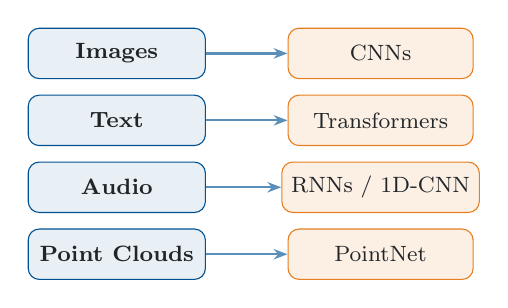
\begin{tikzpicture}[
        modbox/.style={rectangle, draw=UnifiBlue, fill=UnifiBlue!9,
                       rounded corners=4pt, minimum width=2.25cm, minimum height=0.64cm,
                       font=\footnotesize\bfseries, text=UnifiDark},
        archbox/.style={rectangle, draw=AccentOrange, fill=AccentOrange!12,
                        rounded corners=4pt, minimum width=2.35cm, minimum height=0.64cm,
                        font=\footnotesize, text=UnifiDark},
        myarrow/.style={-{Stealth[length=5pt]}, thick, UnifiBlue!65}
      ]
        \node[modbox] (img) at (0,0) {Images};
        \node[modbox] (txt) at (0,-0.85) {Text};
        \node[modbox] (aud) at (0,-1.70) {Audio};
        \node[modbox] (pc)  at (0,-2.55) {Point Clouds};

        \node[archbox] (cnn)   at (3.35,0) {CNNs};
        \node[archbox] (trans) at (3.35,-0.85) {Transformers};
        \node[archbox] (rnn)   at (3.35,-1.70) {RNNs / 1D-CNN};
        \node[archbox] (pnet)  at (3.35,-2.55) {PointNet};

        \draw[myarrow] (img) -- (cnn);
        \draw[myarrow] (txt) -- (trans);
        \draw[myarrow] (aud) -- (rnn);
        \draw[myarrow] (pc)  -- (pnet);
      \end{tikzpicture}
      \end{center}

      \vspace{0.35em}
      \small
      Each data type is usually paired with a dedicated model and
      domain-specific assumptions about structure.
    \end{column}

    \begin{column}{0.40\textwidth}
      {\color{UnifiBlue}\large\bfseries The scaling bottleneck}

      \vspace{0.45em}
      \begin{block}{Self-attention cost}
        \centering
        {\Large $\mathcal{O}(M^2 \cdot d)$}\\[0.2em]
        {\scriptsize grows quadratically with input length $M$}
      \end{block}

      \vspace{0.35em}
      \begin{table}
        \centering\small
        \begin{tabular}{lr}
          \toprule
          \textbf{Input representation} & \textbf{$M$} \\
          \midrule
          $16\!\times\!16$ image patches & $256$ \\
          raw $224\!\times\!224$ pixels & $50{,}176$ \\
          \bottomrule
        \end{tabular}
      \end{table}

      \vspace{0.15em}
      \centering\small
      Raw pixels make standard attention \alert{impractical}.
    \end{column}
  \end{columns}

  \vspace{1.1em}
  {\color{UnifiBlue!25}\hrule height 0.6pt}
  \vspace{0.6em}
  \centering\small
  {\color{UnifiBlue}\textbf{Core question:}}\, can one architecture handle arbitrary inputs without quadratic cost?
\end{frame}

\newcommand{\SolutionCard}[3]{%
  \begin{beamercolorbox}[wd=\linewidth,rounded=true,shadow=true,sep=0pt]{solution card body}
    \begin{beamercolorbox}[wd=\linewidth,rounded=true,sep=0.06cm,leftskip=0.16cm]{solution card title}
      {\normalsize #1}
    \end{beamercolorbox}
    \vspace{0.10em}
    \hspace{0.16cm}\begin{minipage}[t][0.74cm][t]{0.88\linewidth}
      \raggedright
      \hyphenpenalty=10000\exhyphenpenalty=10000
      {\scriptsize\bfseries #2}\\[-0.10em]
      {\scriptsize #3}
    \end{minipage}
    \vspace{0.10em}
  \end{beamercolorbox}%
}

% ── Slide 4: The Perceiver Solution ──────────────────────────────────────────
\begin{frame}[shrink=5]{The Perceiver Solution}
  \setbeamercolor{solution card title}{bg=UnifiBlue, fg=white}
  \setbeamercolor{solution card body}{bg=UnifiBlue!8, fg=UnifiDark}
  \small
  \begin{center}
    \begin{minipage}{0.88\textwidth}
      \centering
      {\color{UnifiBlue}\textbf{Core idea:}} learned latents read the input once; expensive processing stays in latent space.
    \end{minipage}
  \end{center}

  \vspace{0.80em}
  \noindent
  \begin{minipage}[t]{0.29\textwidth}
    \SolutionCard{1. Read}{Cross-attention}{$M$ inputs $\to$ $N \ll M$ latents}
  \end{minipage}\hfill
  \begin{minipage}[t]{0.29\textwidth}
    \SolutionCard{2. Process}{Latent block}{transform $N$ latent slots}
  \end{minipage}\hfill
  \begin{minipage}[t]{0.29\textwidth}
    \SolutionCard{3. Reuse}{Shared weights}{repeat the same processor}
  \end{minipage}

  \vspace{0.22em}
  \begin{center}
    {\color{UnifiDark}\bfseries Complexity shift}

    \vspace{0.18em}
    {\footnotesize Read the full input once; repeat the expensive work in the compact latent space $N \ll M$.}

    \vspace{0.24em}
    \scriptsize
    \renewcommand{\arraystretch}{1.04}
    \begin{tabular*}{0.66\textwidth}{@{\extracolsep{\fill}}lc}
      \toprule
      \textbf{Operation} & \textbf{Cost} \\
      \midrule
      Read input once & $\mathcal{O}(M \cdot N)$ \\
      Process latents for $L$ layers & $\mathcal{O}(L \cdot N^2)$ \\
      \midrule
      \textbf{Perceiver} & $\mathcal{O}(M N + L N^2)$ \\
      \bottomrule
    \end{tabular*}
  \end{center}
\end{frame}

% ── Slide 5: Perceiver IO ───────────────────────────────────────────────────
\section{Perceiver}

\begin{frame}[shrink=5]{Perceiver Architecture}
  \begin{center}
    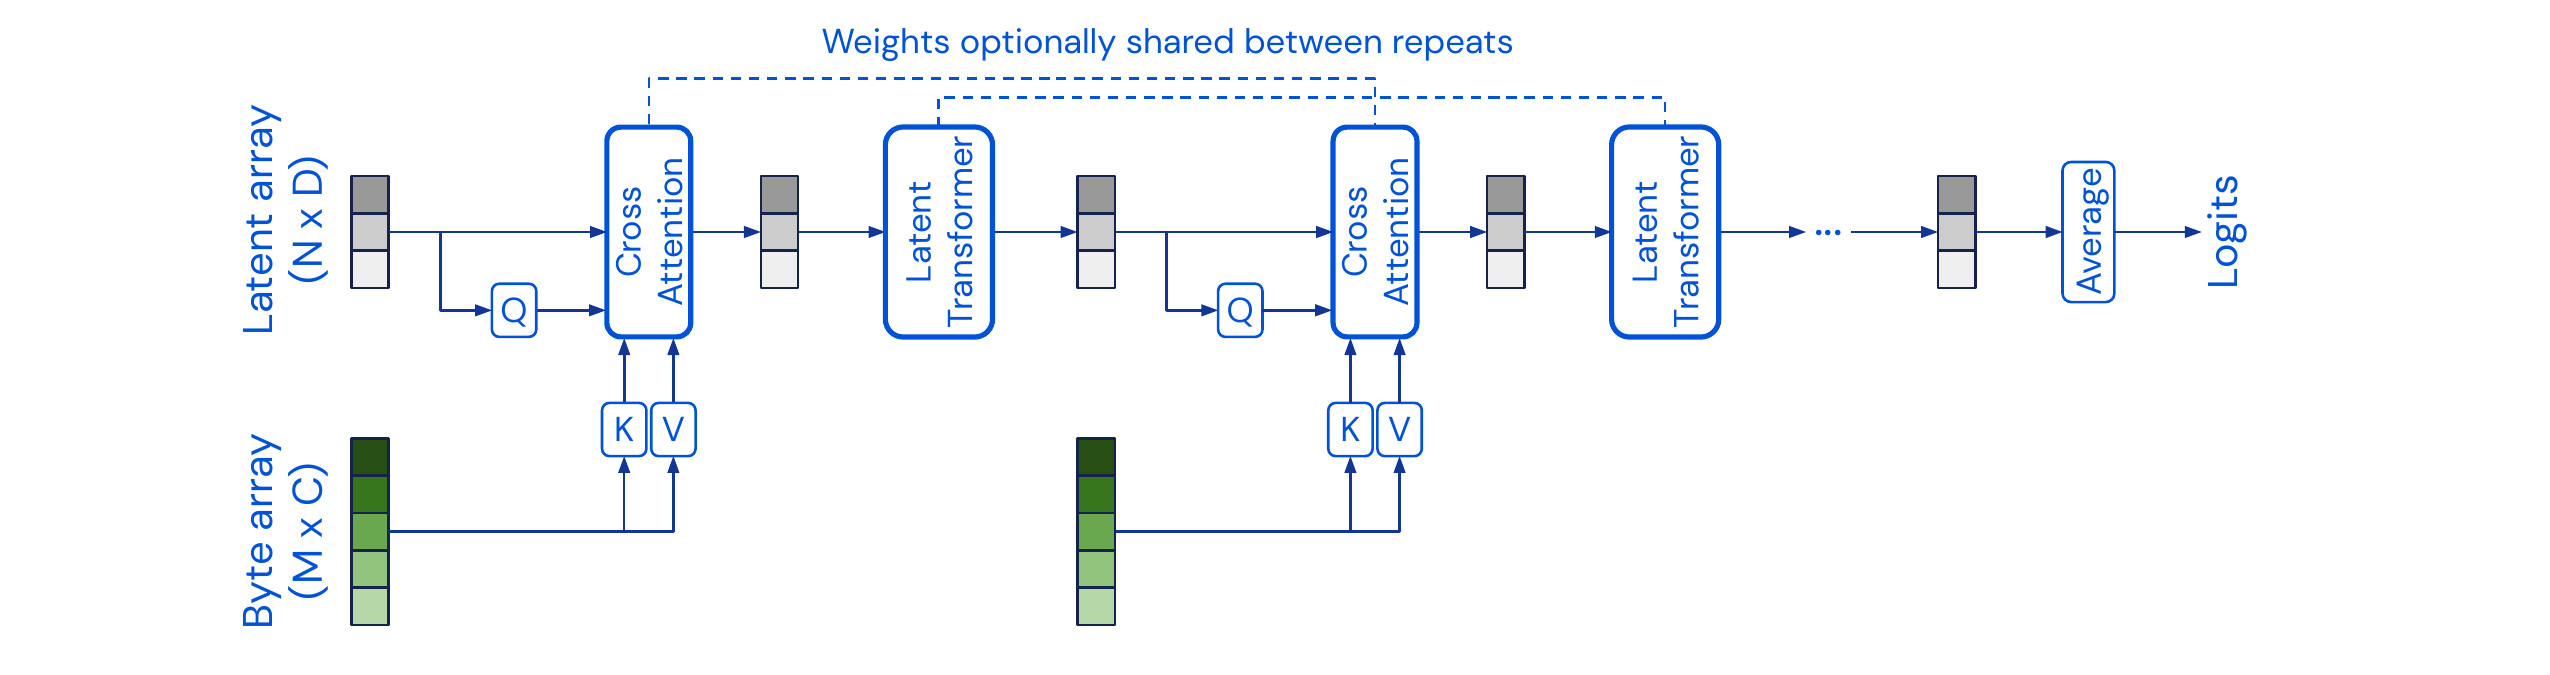
\includegraphics[width=0.98\textwidth,height=0.39\textheight,keepaspectratio]{perceiver_arch.png}
  \end{center}

  \vspace{0em}
  \small
  \begin{columns}[T,onlytextwidth]
    \begin{column}{0.50\textwidth}
      \textbf{Encode and process}
      \begin{itemize}
        \item $X \in \mathbb{R}^{M \times C}$ supplies keys and values.
        \item $Z \in \mathbb{R}^{N \times D}$ supplies queries, with $N \ll M$.
        \item Cross-attention maps $X \rightarrow Z$: $\mathcal{O}(M N)$.
      \end{itemize}
    \end{column}

    \begin{column}{0.46\textwidth}
      \textbf{Latent core and output}
      \begin{itemize}
        \item Latent Transformer updates $Z$ only.
        \item Repeated blocks may share weights.
        \item Original Perceiver pools $Z$; Perceiver IO uses output queries.
      \end{itemize}
    \end{column}
  \end{columns}
\end{frame}

% ══════════════════════════════════════════════════════════════════════════════
% SECTION 2: Architecture (slides 5-13)
% ══════════════════════════════════════════════════════════════════════════════
% Section marker moved before the merged architecture slide.

% ── Slide 6: Architecture Overview ───────────────────────────────────────────
% ── Slide 7: Cross-Attention ─────────────────────────────────────────────────
\begin{frame}{Cross-Attention: The Key Mechanism}
  \begin{columns}[T]
    \begin{column}{0.48\textwidth}
      \textbf{Formally:}
      \begin{align*}
        Q &= X_{\text{latent}} \, W_Q \in \mathbb{R}^{N \times d_k} \\
        K &= X_{\text{input}} \, W_K \in \mathbb{R}^{M \times d_k} \\
        V &= X_{\text{input}} \, W_V \in \mathbb{R}^{M \times d_v}
      \end{align*}
      \[
      \text{CrossAttn}(Q,K,V) = \text{softmax}\!\left(\frac{QK^\top}{\sqrt{d_k}}\right) V
      \]

      \vspace{0.3em}
      The \alert{latents are the queries}, the input provides keys and values $\Rightarrow$ informational \textit{bottleneck}.
    \end{column}
    \begin{column}{0.48\textwidth}
      \begin{center}
        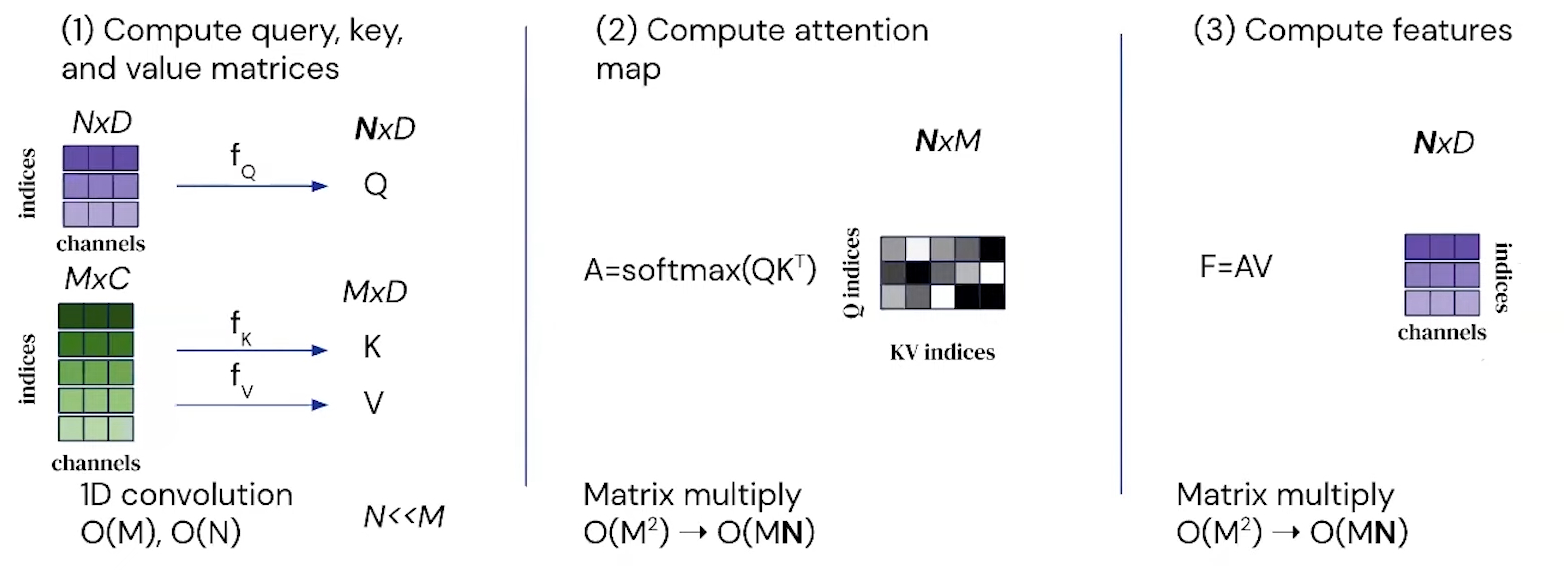
\includegraphics[width=\textwidth,height=0.33\textheight,keepaspectratio]{cross_attention_steps.png}
      \end{center}

      \vspace{0.3em}
      \textbf{Key insight:}
      \begin{itemize}
        \item Attention matrix: $N \times M$ (not $M \times M$)
        \item Complexity: $\mathcal{O}(N \cdot M \cdot d_k)$
        \item Decouples depth from input size
      \end{itemize}
    \end{column}
  \end{columns}
\end{frame}

% ── Slide 8: Latent Transformer & Weight Sharing ─────────────────────────────
\begin{frame}[shrink=3]{Latent Transformer \& Weight Sharing}
  \small
  \textbf{Once information is in the latent array, depth is spent by reusing the same processor on a compact state.}

  \vspace{0.4em}
  \begin{center}
    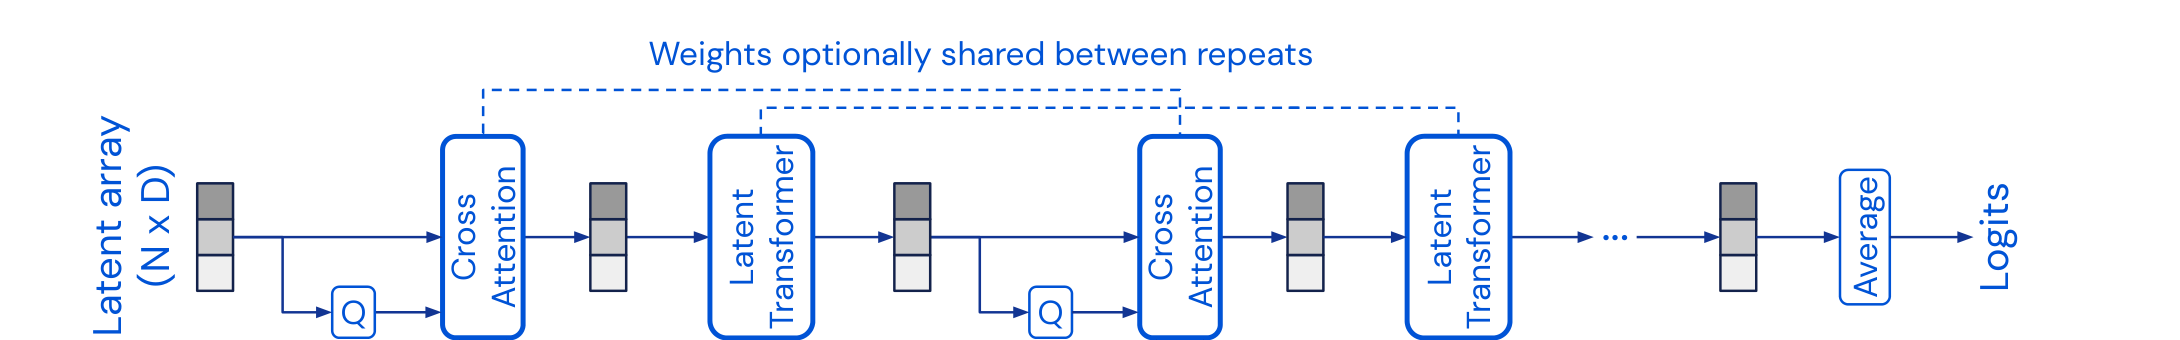
\includegraphics[width=0.97\textwidth,height=0.42\textheight,keepaspectratio]{perceiver_architecture_overview.png}
  \end{center}

  \vspace{0.5em}
  \begin{columns}[T,onlytextwidth]
    \begin{column}{0.48\textwidth}
      \textbf{Weight sharing}
      \begin{itemize}
        \item The same Latent Transformer block $B_{\theta}$ is reused at every repeat, with shared parameters $\theta$.
        \item Unrolling depth behaves like an RNN over the latent state:
          $Z_{t+1}=B_{\theta}(Z_t)$.
      \end{itemize}
    \end{column}

    \begin{column}{0.48\textwidth}
      \textbf{Why it matters}
      \begin{itemize}
        \item Iterative refinement without instantiating a new processor at each step.
        \item Parameter count stays fixed as depth grows; computation stays in the $N$-slot latent space.
      \end{itemize}
    \end{column}
  \end{columns}
\end{frame}

% ── Slide 9: Fourier Positional Encoding ─────────────────────────────────────
\begin{frame}[shrink=3]{Fourier Positional Encoding}
  \small
  \textbf{Perceiver receives a flat array, so location has to be part of each input token.}

  \vspace{0.2em}
  \begin{center}
    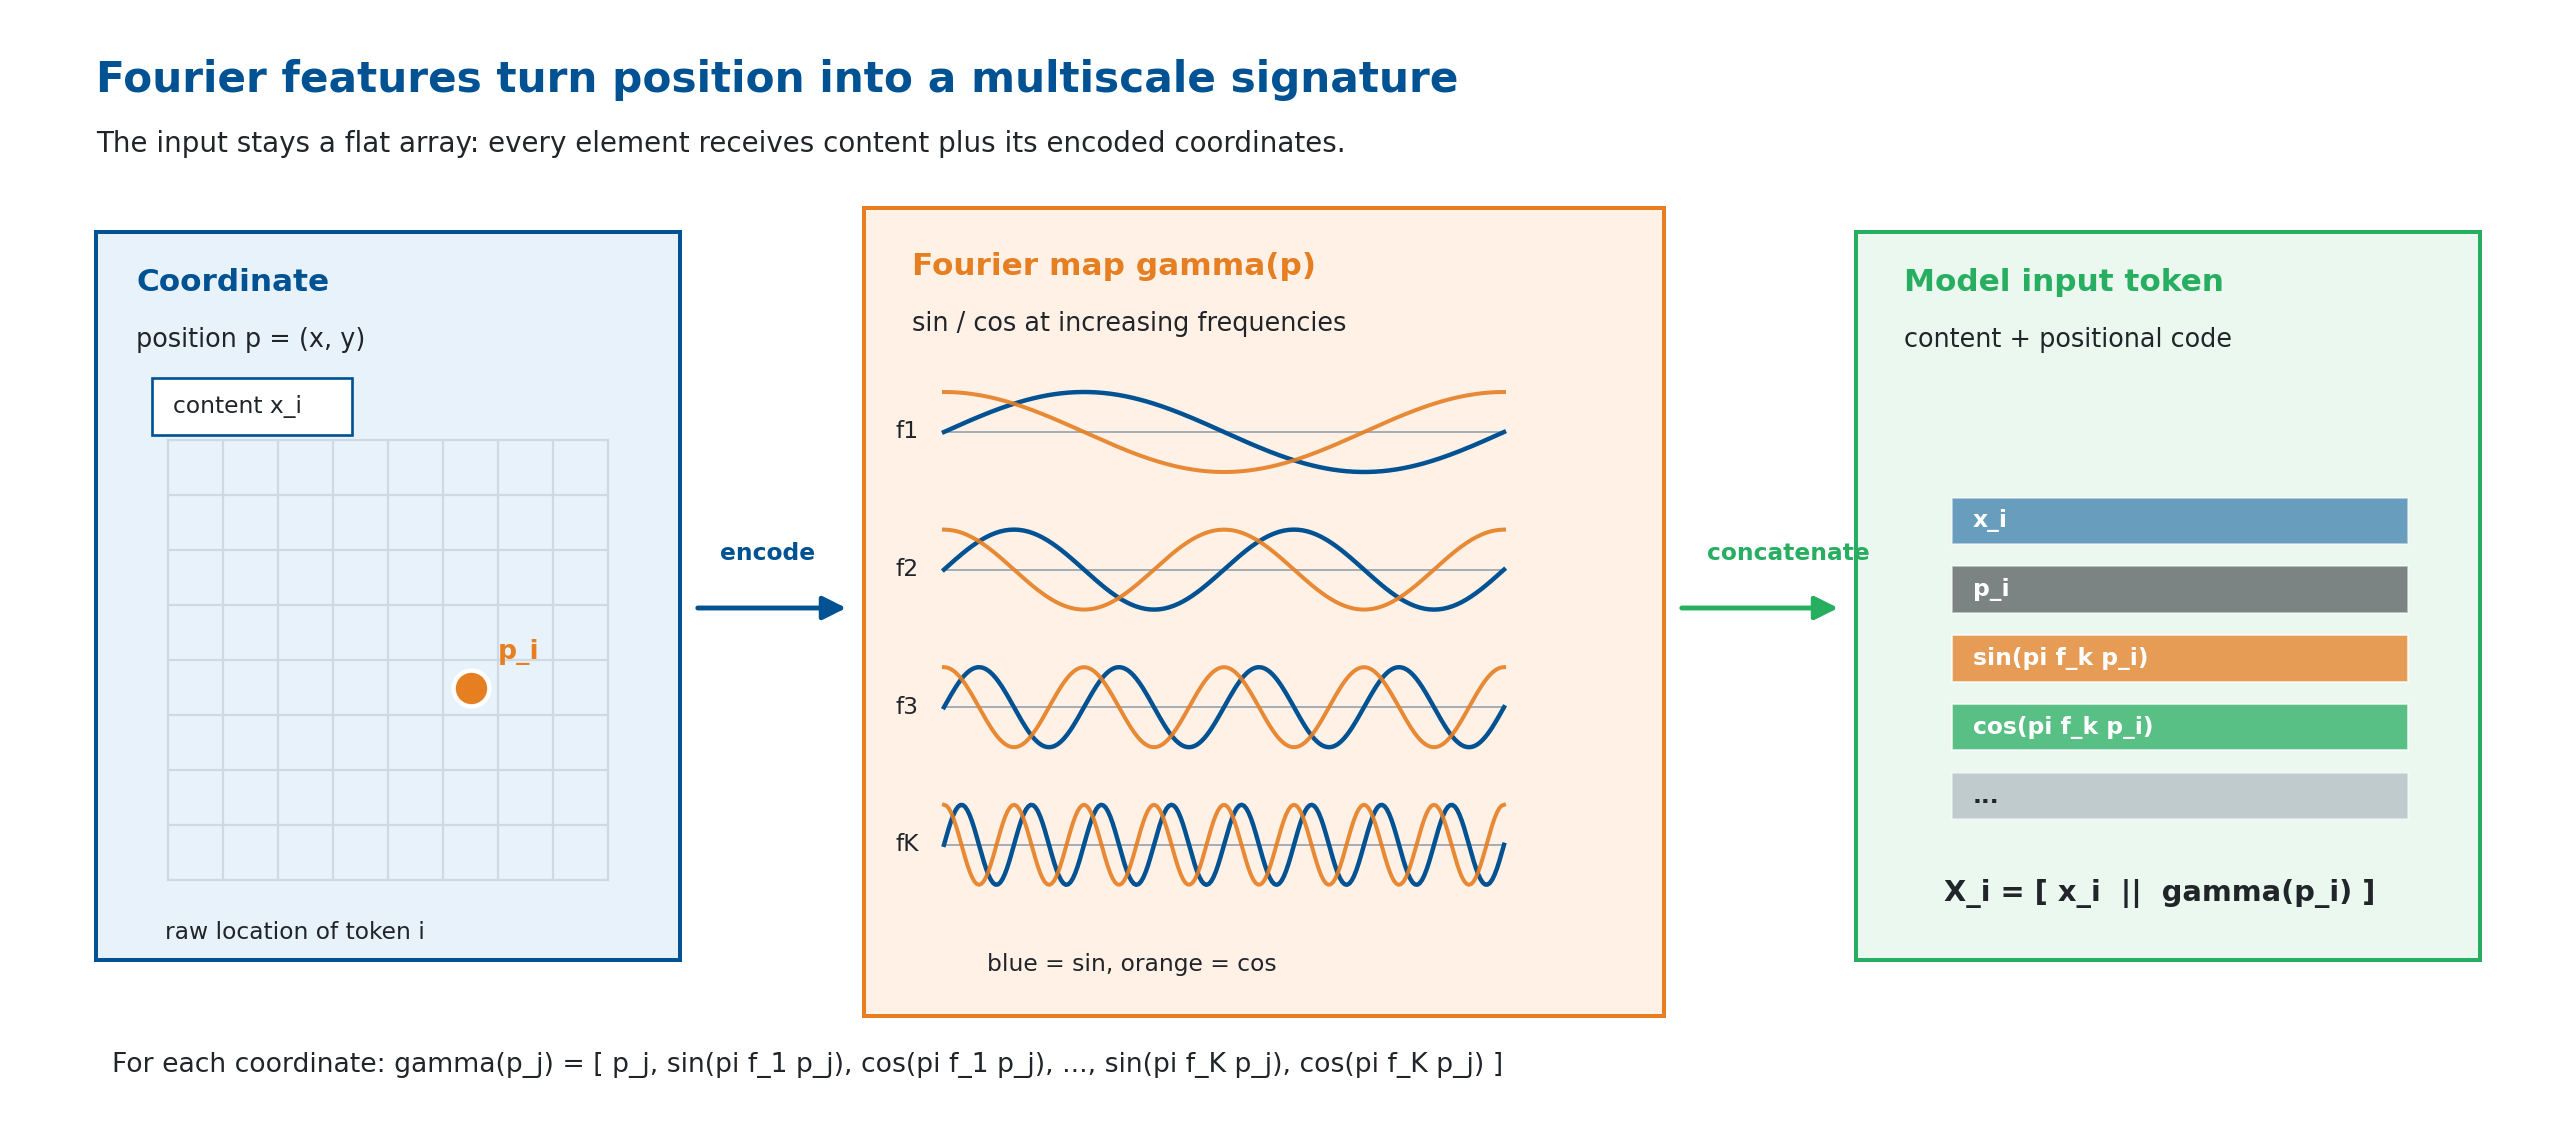
\includegraphics[width=1.0\textwidth,height=0.53\textheight,keepaspectratio]{fourier_features_encoding.png}
  \end{center}

  \vspace{0.35em}
  \begin{columns}[T,onlytextwidth]
    \begin{column}{0.49\textwidth}
      \textbf{General recipe}
      \par\smallskip
      Use domain coordinates: images $(u,v)$, point clouds $(x,y,z)$,
      or text index $t$; sine/cosine bands encode them at multiple scales.
    \end{column}

    \begin{column}{0.47\textwidth}
      \textbf{Input seen by attention}
      \par\smallskip
      The array is still flat, but each token is enriched before projection:
      $X_i=[\,x_i\,\|\,\gamma(p_i)\,]$.
    \end{column}
  \end{columns}
\end{frame}

% ── Slide 10: Perceiver IO Decoder ───────────────────────────────────────────
\begin{frame}[shrink=8]{Perceiver Forward Pass: Shape Checkpoints}
  \begin{columns}[T]
    \begin{column}{0.52\textwidth}
      \textbf{Data flow in the original Perceiver:}
      \begin{enumerate}
        \item Input array: each token stacks content $\mathbf{x}$ with a Fourier position code $\gamma(\mathbf{p})$,
        \[
          X=[\,\mathbf{x}\,\|\,\gamma(\mathbf{p})\,]\in\mathbb{R}^{M\times C}.
        \]
        \item Learned latent array:
        \[
          Z_0\in\mathbb{R}^{N\times D},\qquad N\ll M
        \]
        \item Cross-attention reads input:
        \[
          Q=ZW_Q,\quad K=XW_K,\quad V=XW_V
        \]
        \item Latent Transformer applies self-attention + FFN only on $N$ latents.
      \end{enumerate}
    \end{column}
    \begin{column}{0.44\textwidth}
      \textbf{Shape checkpoints:}
      \begin{table}
        \centering\scriptsize
        \begin{tabular}{lll}
          \toprule
          \textbf{Object} & \textbf{Shape} & \textbf{Meaning} \\
          \midrule
          $X$ & $M\times C$ & input array (content+pos) \\
          $Z_0$ & $N\times D$ & learned latents \\
          $Q$ & $N\times d_k$ & latent queries \\
          $K,V$ & $M\times d_k,d_v$ & input keys/values \\
          $A$ & $N\times M$ & attention map \\
          \bottomrule
        \end{tabular}
      \end{table}

      \vspace{0.4em}
      \begin{block}{Core idea}
        The input size $M$ affects only the cross-attention read; depth is spent in the compact latent space.
      \end{block}
    \end{column}
  \end{columns}
\end{frame}

% ── Slide 11: Output Query Design per Task ───────────────────────────────────
\begin{frame}[shrink=5]{Original Perceiver Output: Pooling Classifier}
  \begin{columns}[T]
    \begin{column}{0.49\textwidth}
      \textbf{Fixed-shape output head:}
      \[
        Z_T=\mathrm{Encoder}(X,Z_0)
      \]
      \[
        z=\frac{1}{N}\sum_{i=1}^{N}Z_T[i]
      \]
      \[
        \mathrm{logits}=zW_{\mathrm{cls}}+b_{\mathrm{cls}}
      \]

      \vspace{0.4em}
      \begin{itemize}
        \item Mean pooling collapses all latents to one vector
        \item The classifier predicts one global label
        \item This is ideal for classification, not dense structured outputs
      \end{itemize}
    \end{column}
    \begin{column}{0.47\textwidth}
      \small
      \textbf{Where FFN and sharing fit:}
      \begin{itemize}
        \item Each latent block is pre-norm attention, residual, FFN, residual
        \item FFN adds non-linearity after attention mixing
        \item Weight sharing repeats the processor over iterations
      \end{itemize}

      \vspace{0.35em}
      \begin{block}{Fixed-shape output}
        Pooling collapses the $N$ latents into a single vector, so this head emits one global prediction per input.
      \end{block}
    \end{column}
  \end{columns}
\end{frame}

% ── Slide 12: Computational Complexity ───────────────────────────────────────
\begin{frame}[shrink=5]{Computational Complexity Analysis}
  \small
  \begin{table}
    \centering\small
    \begin{tabular}{lccc}
      \toprule
      \textbf{Model} & \textbf{Self-Attn} & \textbf{Cross-Attn} & \textbf{Total} \\
      \midrule
      Standard Transformer & $\mathcal{O}(M^2 d)$ & --- & $\mathcal{O}(M^2 d \cdot L)$ \\
      \midrule
      Perceiver & $\mathcal{O}(N^2 d)$ & $\mathcal{O}(MNd)$ & $\mathcal{O}((MN + N^2 L)\,d)$ \\
      \bottomrule
    \end{tabular}
  \end{table}

  \vspace{0.5em}
  \begin{columns}[T]
    \begin{column}{0.48\textwidth}
      \textbf{Symbols:}
      \begin{itemize}
        \item $M$: number of input elements
        \item $N$: number of latent slots, with $N \ll M$
        \item $L$: number of latent processing layers
        \item $d$: hidden channel dimension
      \end{itemize}
    \end{column}
    \begin{column}{0.48\textwidth}
      \textbf{Interpretation:}
      \begin{itemize}
        \item The full input is read through cross-attention
        \item Repeated self-attention happens only in latent space
        \item If $N$ is fixed, depth becomes independent of input length
        \item Concrete sizes are evaluated in the experiments
      \end{itemize}
    \end{column}
  \end{columns}
\end{frame}

% ── Slide 13: GELU & LAMB Optimizer ──────────────────────────────────────────
\section{Experiments: Perceiver}

\begin{frame}[shrink=5]{GELU Activation \& LAMB Optimizer}
  \begin{columns}[T,onlytextwidth]
    \begin{column}{0.48\textwidth}
      \small
      \textbf{GELU (Gaussian Error Linear Unit):}
      \[
      \text{GELU}(x) = x \cdot \Phi(x) \approx x \cdot \sigma(1.702\,x)
      \]
      \vspace{-0.25em}
      \begin{itemize}
        \item Smooth activation used in Transformer architectures
        \item Allows small negative gradient flow
      \end{itemize}

      \vspace{0.2em}
      \textbf{LAMB (Layer-wise Adaptive Moments):}
      \vspace{-0.25em}
      \[
      r_t^{(l)} = \frac{\|w_t^{(l)}\|}{\|w_t^{(l)} + \eta\, \hat{u}_t^{(l)}\|}
      \]
      \vspace{-0.55em}
      {\footnotesize Per-layer trust ratio rescales updates and stabilizes large-batch training.}
    \end{column}
    \begin{column}{0.48\textwidth}
      \small
      \textbf{Why LAMB for Perceiver?}
      \begin{itemize}
        \item Cross-attention bottleneck creates high variance gradients
        \item Standard Adam can \alert{destabilize} with large batches
        \item LAMB safely scales batch sizes up to 1024
      \end{itemize}

      \vspace{0.25em}
      \begin{table}
        \centering\scriptsize
        \begin{tabular}{lcc}
          \toprule
          \textbf{Optimizer} & \textbf{Large Batches} & \textbf{Layer-wise LR} \\
          \midrule
          Adam & Diverges & Global \\
          \textbf{LAMB} & \textbf{Stable} & \textbf{Per-layer trust} \\
          \bottomrule
        \end{tabular}
      \end{table}
    \end{column}
  \end{columns}
\end{frame}

% ── Slide 14: Implementation ─────────────────────────────────────────────────
\begin{frame}[shrink=5]{Implementation}
  \vspace{0.15em}
  \begin{table}
    \centering\scriptsize
    \begin{tabular}{>{\raggedright\arraybackslash}p{0.18\textwidth}>{\raggedright\arraybackslash}p{0.36\textwidth}>{\raggedright\arraybackslash}p{0.36\textwidth}}
      \toprule
      \textbf{Aspect} & \textbf{Paper implementation} & \textbf{Project code} \\
      \midrule
      Core model &
      Cross-attention into learned latents, latent self-attention, FFN, weight sharing &
      Same modules; weight sharing is exposed as an ablation switch \\
      \midrule
      Model scale &
      Large vision/language runs: up to $512{\times}1024$ latents and 201M-param IO &
      Smaller runs: CIFAR-10 $96{\times}384$, ModelNet40/text $128{\times}512$ \\
      \midrule
      Data setting &
      ImageNet, ModelNet40, large language pretraining corpora &
      CIFAR-10, ModelNet40, WikiText-103 byte-level MLM, GLUE fine-tuning \\
      \midrule
      Training budget &
      Distributed accelerators, batches up to 512--1024 &
      Single-GPU budget, batches 32--128, LAMB retained for stability \\
      \midrule
      Practical additions &
      Minimal regularization in the reference setup &
      Dropout, logging, attention-map extraction, and reproducible ablations \\
      \bottomrule
    \end{tabular}
  \end{table}

  \vspace{0.25em}
  {\small The implementation keeps the architectural mechanism intact; the main differences are scale, data budget and training resources.}
\end{frame}

% -- Slide 14b: Implementation Differences from the Paper --
\begin{frame}[shrink=5]{Implementation Differences from the Paper}
  \vspace{0.15em}
  \begin{table}
    \centering\scriptsize
    \begin{tabular}{>{\raggedright\arraybackslash}p{0.20\textwidth}>{\raggedright\arraybackslash}p{0.34\textwidth}>{\raggedright\arraybackslash}p{0.38\textwidth}}
      \toprule
      \textbf{Choice} & \textbf{Original paper (ImageNet)} & \textbf{This project} \\
      \midrule
      Input tokenization &
      Raw pixels, no patching ($M=50{,}176$) &
      \textbf{Raw pixels, no patching} ($M=1{,}024$ on $32{\times}32$) \\
      \addlinespace[2pt]
      Latent array $N\times D$ &
      $512\times1024$ &
      $96\times384$ (CIFAR-10), $128\times512$ (ModelNet40) \\
      \addlinespace[2pt]
      Cross-attend iterations $T$ &
      $8$ &
      $4$ (CIFAR-10), $2$ (ModelNet40) --- and $T$ is itself an ablation axis \\
      \addlinespace[2pt]
      Positional encoding &
      2D Fourier, $K=64$ bands/axis ($258$ dims) &
      \textbf{Identical}: 2D Fourier, $K=64$ bands/axis, $258$ dims $+$ 3 RGB $=261$ \\
      \addlinespace[2pt]
      Weight sharing &
      On by default (shared across $T$) &
      Exposed as an ablation switch (on/off) \\
      \addlinespace[2pt]
      Model selection &
      --- &
      \textbf{Validation carved from train} (45k/5k/10k); test touched once \\
      \addlinespace[2pt]
      Parameters &
      $30$--$200\text{M}+$ &
      $10.18$M (CIFAR-10), $23.29$M (ModelNet40), $18.87$M (IO text) \\
      \bottomrule
    \end{tabular}
  \end{table}

  \vspace{0.3em}
  \begin{block}{Kept identical to the paper}
    \small Core mechanism preserved: cross-attention bottleneck $\to$ weight-shared latent transformer $\to$ mean-pooling (Perceiver) / output-query decoder (IO); GELU MLP, pre-norm LayerNorm, Fourier frequencies linearly spaced to Nyquist.
  \end{block}
\end{frame}

% ══════════════════════════════════════════════════════════════════════════════
% SECTION 3: Experiments & Results (slides 15-28)
% ══════════════════════════════════════════════════════════════════════════════


% ── Slide 15: CIFAR-10 Setup ─────────────────────────────────────────────────
\begin{frame}[shrink=5]{CIFAR-10: Experimental Setup}
  \textbf{Goal:} validate the Perceiver on raw pixels, with no convolutional assumption anywhere.

  \vspace{0.3em}
  \begin{columns}[T]
    \begin{column}{0.46\textwidth}
      \begin{table}
        \centering\small
        \begin{tabular}{ll}
          \toprule
          \textbf{Hyperparameter} & \textbf{Value} \\
          \midrule
          Latent array ($N \times D$) & $96 \times 384$ \\
          Cross-attn stages ($T$) & 4, interleaved \\
          Transformer blocks ($L$) & 4 (shared) \\
          Heads (cross / self) & 1 / 8 \\
          Fourier bands / max freq & 64 / 16 \\
          Dropout & 0 \\
          \midrule
          Optimizer & LAMB \\
          Learning rate & 0.004 \\
          Scheduler & MultiStep 84/102/114 \\
          Batch size & 64 \\
          Epochs & 120, \emph{no early stop} \\
          Precision & bfloat16 \\
          \midrule
          \textbf{Total parameters} & \textbf{10\,175\,362} \\
          \bottomrule
        \end{tabular}
      \end{table}
    \end{column}
    \begin{column}{0.50\textwidth}
      \begin{block}{Protocol --- the part that makes the numbers usable}
        \small
        Train split: \textbf{45\,000} images. Validation: \textbf{5\,000}, carved out of the training set. Test: the official \textbf{10\,000}, touched \emph{once}, at the very end.

        \vspace{0.4em}
        The reported checkpoint is the one with the best \emph{validation} accuracy. Selecting the epoch on the same set you report on is \textbf{selection leakage} and inflates every number.
      \end{block}

      \vspace{0.4em}
      \textbf{Data pipeline}
      \begin{itemize}
        \item $32\!\times\!32$ RGB image $\to$ \textbf{1\,024 pixels} as an unordered set
        \item Each pixel: 3 RGB $+$ 2D Fourier PE $= $ \textbf{261 dims} --- the same per-pixel width as the paper
        \item No patching, no convolution, no learned tokenizer
      \end{itemize}
    \end{column}
  \end{columns}
\end{frame}

% ── The noise band ───────────────────────────────────────────────────────────
\begin{frame}[shrink=5]{The Noise Band: How Much Does a Number Move on Its Own?}
  \begin{columns}[T]
    \begin{column}{0.52\textwidth}
      \textbf{Three runs, identical in everything but the seed:}
      \begin{table}
        \centering\small
        \begin{tabular}{llc}
          \toprule
          \textbf{Run} & \textbf{Seed} & \textbf{Test acc.} \\
          \midrule
          \texttt{e01\_baseline} & 42 & 71.63\% \\
          \texttt{e31\_baseline\_seed1} & 1 & 68.85\% \\
          \texttt{e32\_baseline\_seed2} & 2 & 70.97\% \\
          \midrule
          \multicolumn{2}{l}{\textbf{Spread (max $-$ min)}} & \textbf{2.78pp} \\
          \bottomrule
        \end{tabular}
      \end{table}

      \vspace{0.3em}
      \begin{alertblock}{The rule for every slide that follows}
        \small
        Any difference smaller than \textbf{2.78 percentage points} is not an effect. It is seed variance.
      \end{alertblock}
    \end{column}
    \begin{column}{0.44\textwidth}
      \begin{block}{Why this slide exists}
        \small
        Two extra runs cost a few GPU-hours and change the status of all the others: without a measured band, every comparison is an opinion.

        \vspace{0.4em}
        It also sets the honest ceiling of this study. On CIFAR-10 with 1\,024 pixels and one GPU, most of the paper's ablations --- measured on ImageNet with 50\,176 pixels and 64 TPUs --- simply do not have room to show up.
      \end{block}

      \vspace{0.3em}
      \scriptsize The band depends on the metric: 2.78pp on test accuracy, 2.94pp on best validation, 3.24pp on final validation. The conclusions do not change.
    \end{column}
  \end{columns}
\end{frame}

% ── Ablation overview ────────────────────────────────────────────────────────
\begin{frame}[shrink=4]{CIFAR-10: What Survives the Noise Band}
  \begin{columns}[T,onlytextwidth]
    \begin{column}{0.70\textwidth}
      
\includegraphics[width=\textwidth,height=0.80\textheight,keepaspectratio]{cifar10_ablation_correct.png}
    \end{column}
    \begin{column}{0.27\textwidth}
      \textbf{23 runs, 11 conclusive}

      \vspace{0.3em}
      \begin{itemize}
        \item \textcolor{AccentOrange}{\textbf{Outside}} the band: latent init scale, cross-attend arrangement, Fourier bands, no latent transformer
        \item \textcolor{gray}{\textbf{Inside}}: permutation, learned PE, weight sharing, max frequency
      \end{itemize}

      \vspace{0.2em}
      {\scriptsize Source: \texttt{test\_accuracy} at \texttt{selected\_epoch}, read from \texttt{logs/<run>/results.json}.}
    \end{column}
  \end{columns}
\end{frame}

% ── Permutation ──────────────────────────────────────────────────────────────
\begin{frame}[shrink=5]{CIFAR-10: Permutation Invariance --- the Headline Claim}
  \begin{table}
    \centering\small
    \begin{tabular}{llcc}
      \toprule
      \textbf{Comparison} & \textbf{Positional encoding} & \textbf{Natural $\to$ permuted} & \textbf{$\Delta$} \\
      \midrule
      \texttt{e01} $\to$ \texttt{e02} & Fourier & $71.63\% \to 68.95\%$ & $-2.68$ \\
      \texttt{e03} $\to$ \texttt{e04} & learned & $71.07\% \to 69.87\%$ & $-1.20$ \\
      \midrule
      \multicolumn{4}{l}{\textit{Paper (ImageNet):} Fourier $78.0 \to 78.0$ \quad learned $70.9 \to 70.9$} \\
      \bottomrule
    \end{tabular}
  \end{table}

  \vspace{0.4em}
  \begin{columns}[T]
    \begin{column}{0.48\textwidth}
      \begin{block}{What we measured}
        \small
        Both drops fall \textbf{inside} the 2.78pp band: shuffling the pixels causes no measurable damage. Invariance confirmed --- in the honest, weak form: \emph{we did not measure a loss}, which is not the same as proving the loss is zero.
      \end{block}
    \end{column}
    \begin{column}{0.48\textwidth}
      \begin{block}{The subtle point}
        \small
        Invariance holds for \textbf{both} encodings. It comes from \textbf{attention} --- a weighted sum has no order --- not from the Fourier features. Fourier features buy \emph{absolute} accuracy on ImageNet (78.0 vs 70.9), because learning 50\,176 distinct positional embeddings is hard; they are not what makes the model permutation-proof.
      \end{block}
    \end{column}
  \end{columns}
\end{frame}

% ── Capacity ─────────────────────────────────────────────────────────────────
\begin{frame}[shrink=4]{CIFAR-10: Capacity Does Not Buy Accuracy}
  \begin{columns}[T,onlytextwidth]
    \begin{column}{0.58\textwidth}
      
\includegraphics[width=\textwidth,height=0.66\textheight,keepaspectratio]{weight_sharing_tradeoff_correct.png}
    \end{column}
    \begin{column}{0.38\textwidth}
      \textbf{Weight sharing is free}
      \begin{itemize}\small
        \item \texttt{e01} 71.63\% with 10.2M params
        \item \texttt{e16} 69.46\% with \textbf{31.5M} params
        \item $3.1\times$ the weights, \textcolor{AccentRed}{$-$2.17pp} --- inside the band
      \end{itemize}

      \vspace{0.4em}
      \textbf{Where you put capacity matters}
      \begin{itemize}\small
        \item Remove the latent transformer, add cross-attends instead:
        \item 6.1M $\to$ 68.98\% \\ 12.2M $\to$ 67.24\% \\ 18.3M $\to$ 67.05\%
        \item \textcolor{AccentRed}{\textbf{More parameters, less accuracy}}
      \end{itemize}
    \end{column}
  \end{columns}
\end{frame}

% ── Tab. 6 ───────────────────────────────────────────────────────────────────
\begin{frame}[shrink=5]{CIFAR-10: How Many Cross-Attends, and Where}
  \begin{table}
    \centering\small
    \begin{tabular}{lccc}
      \toprule
      \textbf{$T$} & \textbf{interleaved} & \textbf{all at start} & \textbf{$\Delta$ (arrangement)} \\
      \midrule
      1 & \textbf{72.91\%} & \textbf{72.91\%} & $0.00$ \\
      2 & 66.23\% & 68.45\% & $+2.22$ \\
      4 & \textbf{71.63\%} \tiny(baseline) & 67.19\% & \textcolor{AccentRed}{$\mathbf{-4.44}$} \\
      8 & 65.63\% & 68.04\% & $+2.41$ \\
      \bottomrule
    \end{tabular}
  \end{table}

  \vspace{0.3em}
  \begin{columns}[T]
    \begin{column}{0.48\textwidth}
      \begin{block}{The one conclusive result}
        \small
        At $T=4$, interleaving beats front-loading by \textbf{4.44pp} --- outside the band. Re-reading the input \emph{after} the latents have been refined lets each pass look for something different.
      \end{block}
    \end{column}
    \begin{column}{0.48\textwidth}
      \begin{block}{A reproducibility check, for free}
        \small
        At $T=1$ the two arrangements produce the \emph{same computational graph}, and indeed give bit-identical results: 72.91\%, epoch 90, 8\,654\,662 params. Fixed seed $\Rightarrow$ reproducible training.
      \end{block}
    \end{column}
  \end{columns}

  \vspace{0.2em}
  \scriptsize Note the non-monotonicity along $T$: reading the input once is as good as reading it four times, with 15\% fewer parameters.
\end{frame}

% ── Fig. 6 ───────────────────────────────────────────────────────────────────
\begin{frame}[shrink=5]{CIFAR-10: The Hyperparameter That Actually Matters}
  \begin{columns}[T]
    \begin{column}{0.50\textwidth}
      \begin{table}
        \centering\small
        \begin{tabular}{lcc}
          \toprule
          \textbf{Sweep} & \textbf{Value} & \textbf{Test acc.} \\
          \midrule
          \multirow{3}{*}{Latent init $\sigma$}
            & \textbf{0.02} & \textbf{71.63\%} \\
            & 0.1 & \textcolor{AccentOrange}{65.69\%} \\
            & 1.0 & \textcolor{AccentRed}{\textbf{52.08\%}} \\
          \midrule
          \multirow{3}{*}{Fourier bands}
            & 4 & 66.39\% \\
            & 16 & 62.58\% \\
            & \textbf{64} & \textbf{71.63\%} \\
          \midrule
          \multirow{3}{*}{Max frequency}
            & 8 & 69.50\% \\
            & \textbf{16} & \textbf{71.63\%} \\
            & 64 & 72.41\% \\
          \bottomrule
        \end{tabular}
      \end{table}
    \end{column}
    \begin{column}{0.46\textwidth}
      \begin{alertblock}{Latent initialisation: the only clean monotone effect}
        \small
        $\sigma$ from 0.02 to 1.0 costs \textbf{19.55pp}. At $\sigma=1.0$ the best epoch is \textbf{9 out of 120}: the model learns briefly, then degrades for the remaining 111 epochs.
      \end{alertblock}

      \vspace{0.3em}
      \begin{block}{Two honest caveats}
        \scriptsize
        \textbf{Bands} is non-monotone (4 beats 16), and both low points are runs whose \emph{final} validation collapsed (22.5\% and 55.5\%) --- an optimisation problem, not a resolution one.

        \vspace{0.3em}
        \textbf{Max frequency} sits entirely inside the noise band. The whole axis is inconclusive, and saying so is part of the result.
      \end{block}
    \end{column}
  \end{columns}
\end{frame}

% ── ModelNet40 ───────────────────────────────────────────────────────────────
\begin{frame}[shrink=5]{ModelNet40: Same Network, 3D Point Clouds}
  \begin{columns}[T]
    \begin{column}{0.44\textwidth}
      \begin{table}
        \centering\small
        \begin{tabular}{ll}
          \toprule
          \textbf{Setting} & \textbf{Value} \\
          \midrule
          Latent array & $128 \times 512$ \\
          Cross-attn / blocks & 2 / 6 \\
          Points per model & 2\,048 \\
          Input per point & 387 dims \\
          Fourier bands / max f & 64 / 1120 \\
          Optimizer / lr & LAMB / 0.001 \\
          Batch (paper: 512) & \textbf{32} \\
          Epochs & 120 \\
          Parameters & 23\,288\,928 \\
          \bottomrule
        \end{tabular}
      \end{table}

      \vspace{0.2em}
      \scriptsize \textbf{Metric note:} ModelNet40 has no separate validation split --- the standard test set (2\,468 objects) \emph{is} the validation set, so the figure is \texttt{val\_accuracy} at the best epoch.
    \end{column}
    \begin{column}{0.52\textwidth}
      
\includegraphics[width=\textwidth,height=0.60\textheight,keepaspectratio]{modelnet40_correct.png}

      \vspace{0.2em}
      \begin{block}{Above the paper}
        \small
        \textbf{87.36\%} vs the paper's \textbf{85.7\%}, with a batch $16\times$ smaller. Plausible: ModelNet40 is small and its objects arrive canonically aligned, so the large-batch advantage that dominates ImageNet counts for little here.
      \end{block}
    \end{column}
  \end{columns}
\end{frame}

% ── ModelNet40 augmentation ──────────────────────────────────────────────────
\begin{frame}[shrink=5]{ModelNet40: Rotation Costs 13 Points --- and Why}
  \begin{columns}[T]
    \begin{column}{0.46\textwidth}
      \begin{table}
        \centering\small
        \begin{tabular}{lcc}
          \toprule
          \textbf{Augmentation} & \textbf{Accuracy} & \textbf{$\Delta$} \\
          \midrule
          scale only & \textbf{87.36\%} & --- \\
          $+$ translation & 87.20\% & $-0.16$ \\
          $+$ rotation & \textcolor{AccentRed}{74.07\%} & \textcolor{AccentRed}{\textbf{$-13.29$}} \\
          \bottomrule
        \end{tabular}
      \end{table}

      \vspace{0.4em}
      \begin{block}{The largest effect in the whole project}
        \small
        And the one with the cleanest theoretical explanation.
      \end{block}
    \end{column}
    \begin{column}{0.50\textwidth}
      \begin{block}{The Perceiver has no rotational inductive bias}
        \small
        3D Fourier PE encodes \textbf{absolute} position. Rotating an object changes every coordinate --- and therefore every encoding --- while the label stays the same. The network must learn from scratch an invariance the architecture does not grant, and that this task does not even need: ModelNet40 objects are already canonically aligned.

        \vspace{0.4em}
        Translation is nearly harmless ($-0.16$) because it shifts all points equally: the \emph{relative} structure survives.
      \end{block}

      \vspace{0.2em}
      \scriptsize \textbf{Takeaway:} a missing inductive bias cannot be patched with augmentation.
    \end{column}
  \end{columns}
\end{frame}

\section{Perceiver IO}

% -- Perceiver IO: Structured Outputs ------------------------------------------------
\begin{frame}[shrink=5]{Perceiver IO: Structured Outputs}
  \begin{center}
    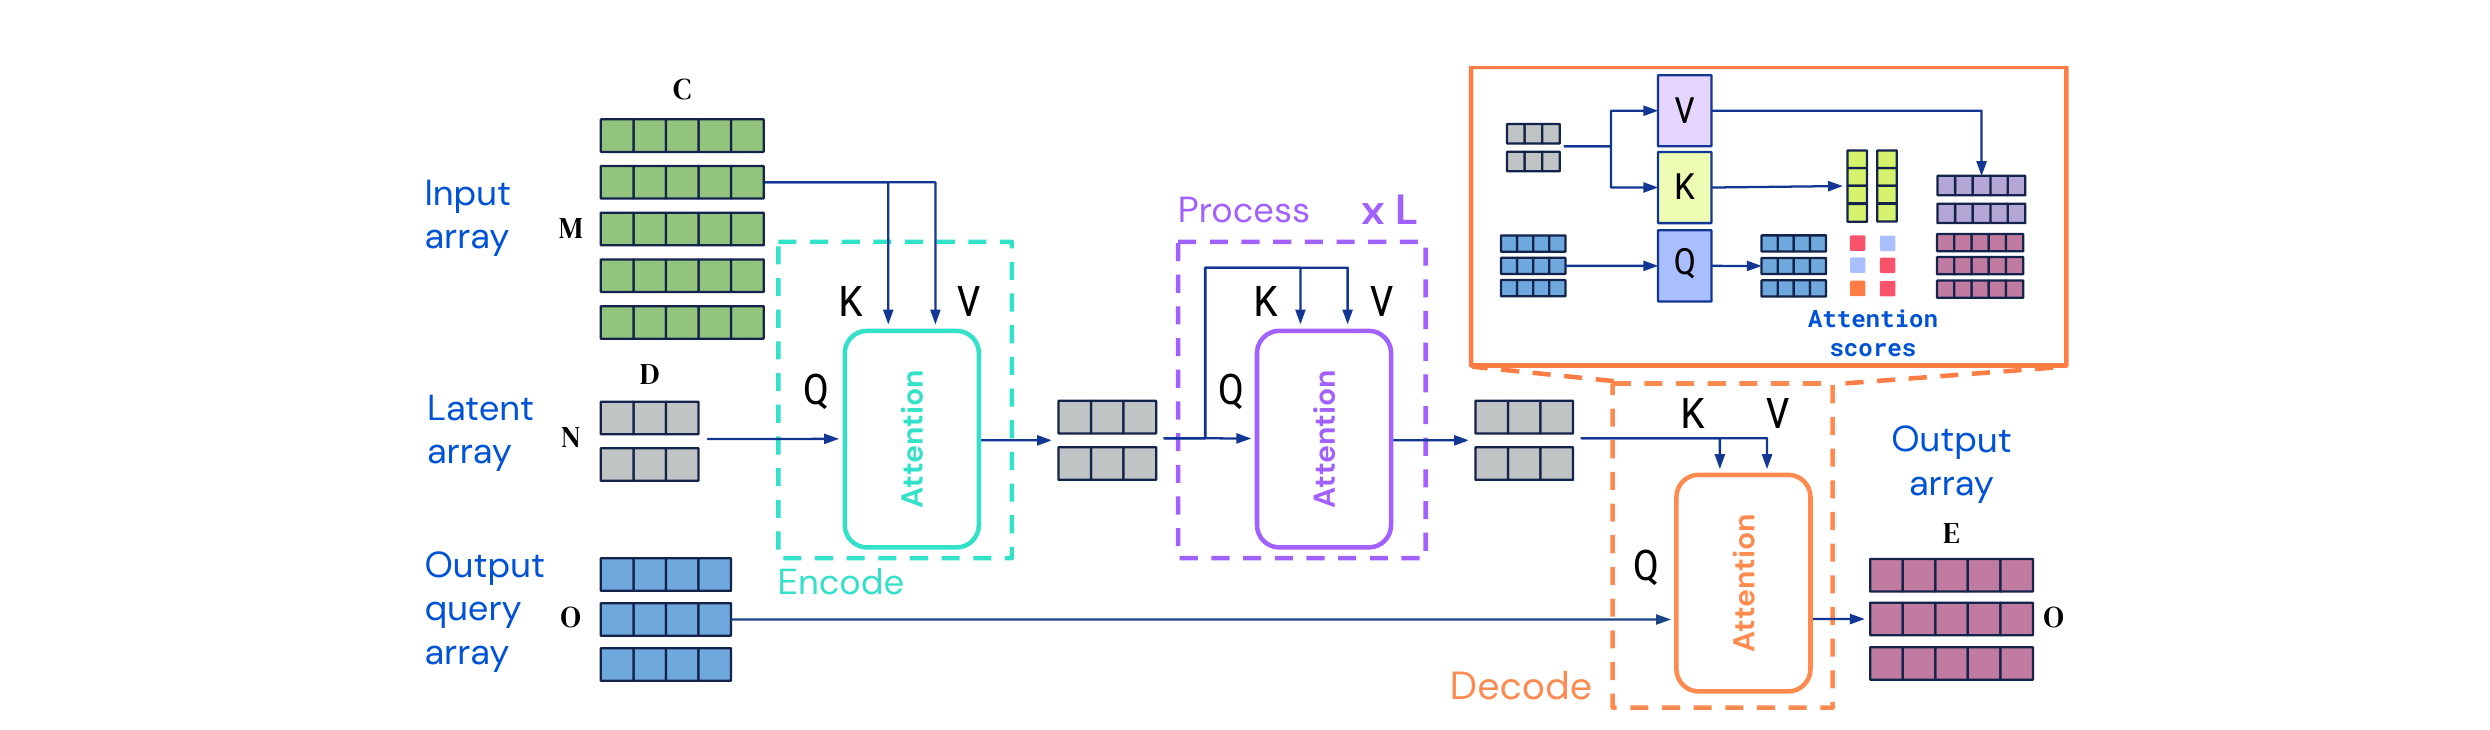
\includegraphics[width=0.95\textwidth,height=0.40\textheight,keepaspectratio]{perceiverio_arch.png}
  \end{center}

  \vspace{0.15em}
  \begin{columns}[T,onlytextwidth]
    \begin{column}{0.48\textwidth}
      \small
      \textbf{Extension over Perceiver} (Jaegle et al., ICLR 2022):
      \begin{itemize}
        \item \textbf{Encode}: input $\rightarrow$ latent (same cross-attn encoder)
        \item \textbf{Process}: latent self-attention ($\times L$)
        \item \textbf{Decode}: \alert{output queries} read latents
      \end{itemize}
    \end{column}
    \begin{column}{0.48\textwidth}
      \small
      \textbf{Why it matters:}
      \begin{itemize}
        \item Original Perceiver: one pooled global output
        \item IO: task-specific output shape
        \item Same latent bottleneck, more general decoder
      \end{itemize}
    \end{column}
  \end{columns}
\end{frame}

% -- Perceiver IO Decoder ------------------------------------------------------------
\begin{frame}[shrink=12]{Perceiver IO Decoder with Output Queries}
  \begin{center}
    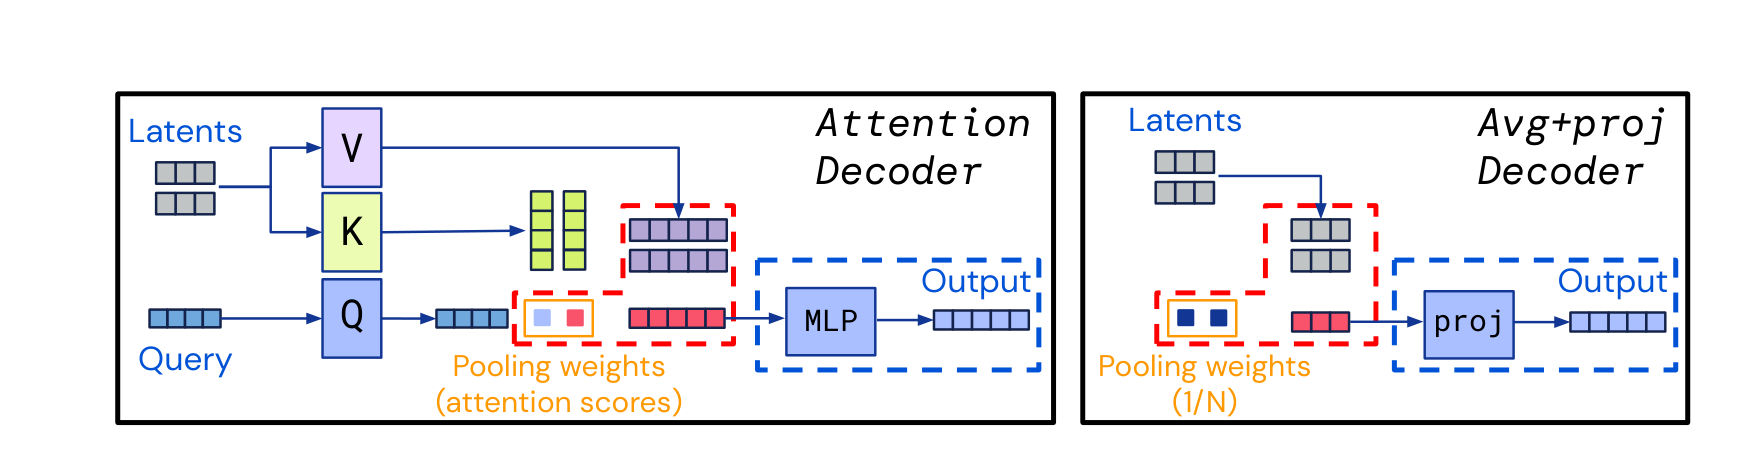
\includegraphics[width=0.86\textwidth,height=0.31\textheight,keepaspectratio]{perceiver_io_decoder.png}
  \end{center}

  \vspace{0.25em}
  \textbf{Decoder cross-attention (single layer):}
  \[
  Q_{\text{dec}} = \text{OutputQuery}\,W_Q, \quad
  K_{\text{dec}} = \text{Latent}\,W_K, \quad
  V_{\text{dec}} = \text{Latent}\,W_V
  \]
  \[
  \text{Output} = \text{softmax}\!\left(\frac{Q_{\text{dec}} K_{\text{dec}}^\top}{\sqrt{d_k}}\right) V_{\text{dec}} \in \mathbb{R}^{O \times E}
  \]

  \vspace{0.3em}
  \begin{itemize}
    \item The number of output queries $O$ is \textbf{task-dependent} and independent of $N$ and $M$
    \item A single decoder cross-attention layer suffices (no self-attention among outputs)
  \end{itemize}
\end{frame}

% -- Output Query Design -------------------------------------------------------------
\begin{frame}[shrink=4]{Output Query Design per Task}
  \begin{center}
  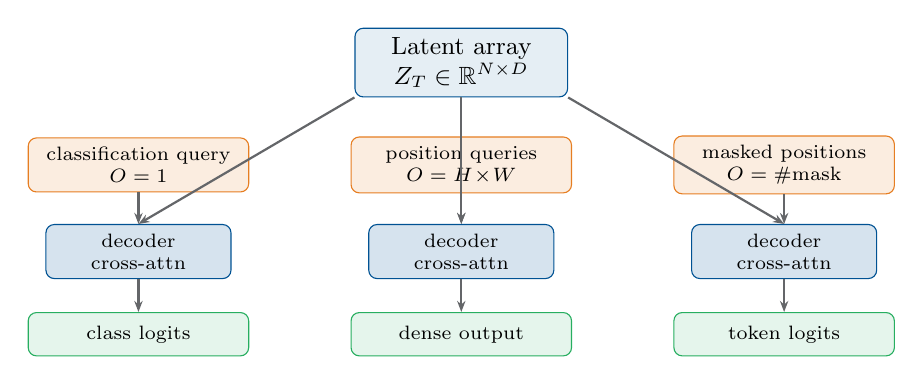
\begin{tikzpicture}[
    latent/.style={rectangle, draw=UnifiBlue, fill=UnifiBlue!10,
                   rounded corners=3pt, minimum width=2.7cm,
                   minimum height=0.62cm, align=center, font=\small},
    query/.style={rectangle, draw=AccentOrange, fill=AccentOrange!14,
                  rounded corners=3pt, minimum width=2.8cm,
                  minimum height=0.55cm, align=center, font=\scriptsize},
    dec/.style={rectangle, draw=UnifiBlue, fill=UnifiBlue!16,
                rounded corners=3pt, minimum width=2.35cm,
                minimum height=0.55cm, align=center, font=\scriptsize},
    outbox/.style={rectangle, draw=AccentGreen, fill=AccentGreen!12,
                   rounded corners=3pt, minimum width=2.8cm,
                   minimum height=0.55cm, align=center, font=\scriptsize},
    arr/.style={-{Stealth[length=4pt]}, thick, UnifiDark!70}
  ]
    \node[latent] (lat) at (0,1.65) {Latent array\\$Z_T \in \mathbb{R}^{N\times D}$};

    \node[query] (q1) at (-4.1,0.35) {classification query\\$O=1$};
    \node[query] (q2) at (0,0.35) {position queries\\$O=H\!\times\!W$};
    \node[query] (q3) at (4.1,0.35) {masked positions\\$O=\#\mathrm{mask}$};

    \node[dec] (d1) at (-4.1,-0.75) {decoder\\cross-attn};
    \node[dec] (d2) at (0,-0.75) {decoder\\cross-attn};
    \node[dec] (d3) at (4.1,-0.75) {decoder\\cross-attn};

    \node[outbox] (o1) at (-4.1,-1.80) {class logits};
    \node[outbox] (o2) at (0,-1.80) {dense output};
    \node[outbox] (o3) at (4.1,-1.80) {token logits};

    \draw[arr] (q1) -- (d1);
    \draw[arr] (q2) -- (d2);
    \draw[arr] (q3) -- (d3);
    \draw[arr] (d1) -- (o1);
    \draw[arr] (d2) -- (o2);
    \draw[arr] (d3) -- (o3);
    \draw[arr] (lat.south west) -- (d1.north);
    \draw[arr] (lat.south) -- (d2.north);
    \draw[arr] (lat.south east) -- (d3.north);
  \end{tikzpicture}
  \end{center}

  \vspace{0.2em}
  \begin{columns}[T,onlytextwidth]
    \begin{column}{0.31\textwidth}
      \begin{block}{Classification}
        \scriptsize One learned query produces one global prediction.
      \end{block}
    \end{column}
    \begin{column}{0.31\textwidth}
      \begin{block}{Dense outputs}
        \scriptsize Output shape is controlled by the query array.
      \end{block}
    \end{column}
    \begin{column}{0.31\textwidth}
      \begin{block}{Masked LM}
        \scriptsize Only masked positions need decoder queries.
      \end{block}
    \end{column}
  \end{columns}
\end{frame}



\section{Experiments: Perceiver IO}

% -- CIFAR comparison after IO explanation ------------------------------------------
\begin{frame}[shrink=5]{Perceiver IO on CIFAR-10: Not Yet Measured}
  \begin{columns}[T]
    \begin{column}{0.50\textwidth}
      \begin{block}{The question these runs will answer}
        \small
        Same encoder as \texttt{e01\_baseline}, but the mean-pooling head is replaced by a \textbf{decoder with one output query}.

        \vspace{0.4em}
        \texttt{io01\_cifar} and its seed replica \texttt{io02\_cifar\_seed1} are in the registry; \textbf{neither has been run}.
      \end{block}

      \vspace{0.3em}
      \begin{block}{What to expect, honestly}
        \small
        Very little. The query decoder earns its keep when the output is \textbf{structured} --- a segmentation mask, an optical-flow field, 1\,024 tokens. For a single label out of ten, querying the latents and averaging them should be equivalent.

        \vspace{0.3em}
        The interesting outcome would be \emph{no difference}: evidence that the decoder generalises the output shape at no cost in the simple case.
      \end{block}
    \end{column}
    \begin{column}{0.46\textwidth}
      \begin{alertblock}{A number that used to be on this slide}
        \small
        Earlier versions of this deck reported \textbf{Perceiver IO 78.20\% vs Perceiver 69.69\%}, concluding the decoder was worth \textbf{$+$8.51pp}.

        \vspace{0.4em}
        That comparison came from a first-generation run in which the \textbf{test set was also used as validation}, and in which three ablation flags were never read by the code.

        \vspace{0.4em}
        It has been \textbf{removed, not updated}. Replacing it with an estimate would have meant inventing a result.
      \end{alertblock}

      \vspace{0.3em}
      \scriptsize Paper reference (ImageNet): Perceiver IO \textbf{79.0\%} with 2D Fourier features, \textbf{84.5\%} with JFT pre-training --- never using a convolution.
    \end{column}
  \end{columns}
\end{frame}

% ── MLM ──────────────────────────────────────────────────────────────────────
\begin{frame}[shrink=5]{WikiText-103: Byte-Level Masked Language Model}
  \begin{columns}[T]
    \begin{column}{0.46\textwidth}
      \begin{table}
        \centering\small
        \begin{tabular}{ll}
          \toprule
          \textbf{Setting} & \textbf{Value} \\
          \midrule
          Latent array & $128 \times 512$ \\
          Cross-attn / blocks & 1 / 4 \\
          Heads (cross / self) & 1 / 8 \\
          Sequence length & 512 bytes \\
          Vocabulary & $256 + 1$ mask \\
          Masking rate & 15\% \\
          Output queries & one per position \\
          Optimizer / lr & LAMB / 0.001 \\
          Epochs / batch & 10 / 32 \\
          Parameters & 18\,872\,740 \\
          \midrule
          \textbf{Masked-byte accuracy} & \textbf{86.68\%} \\
          Chance level ($1/256$) & 0.39\% \\
          \bottomrule
        \end{tabular}
      \end{table}
    \end{column}
    \begin{column}{0.50\textwidth}
      \begin{block}{The only real Perceiver IO result --- and it is solid}
        \small
        \textbf{$\sim$222$\times$ better than chance}, reading raw UTF-8 with \textbf{no tokenizer at all}. Nearly nine masked bytes out of ten reconstructed.
      \end{block}

      \vspace{0.3em}
      \begin{block}{Why bytes are affordable here}
        \small
        Cross-attention costs $O(M \cdot N)$ --- \emph{linear} in sequence length --- instead of $O(M^2)$. Going from 512 tokens to 2\,048 bytes costs BERT $16\times$ in attention, and Perceiver IO only $4\times$.
      \end{block}

      \vspace{0.3em}
      \begin{alertblock}{Read this number carefully}
        \scriptsize
        Masked-\emph{byte} accuracy is not comparable to masked-\emph{token} accuracy: the space is 256 rather than tens of thousands, and many bytes are fixed by orthographic context. It shows the pre-training worked. It is not a comparison with BERT --- that comparison lives on GLUE.
      \end{alertblock}
    \end{column}
  \end{columns}
\end{frame}

% ── GLUE ─────────────────────────────────────────────────────────────────────
\begin{frame}[shrink=5]{GLUE: Protocol Ready, Runs Pending}
  \begin{columns}[T]
    \begin{column}{0.52\textwidth}
      \begin{table}
        \centering\scriptsize
        \begin{tabular}{llcc}
          \toprule
          \textbf{Run} & \textbf{Task} & \textbf{Ep.} & \textbf{Majority} \\
          \midrule
          \texttt{io\_glue\_cola} & acceptability & 30 & $\approx$69\% \\
          \texttt{io\_glue\_sst2} & sentiment & 10 & $\approx$50\% \\
          \texttt{io\_glue\_mrpc} & paraphrase & 30 & $\approx$68\% \\
          \texttt{io\_glue\_stsb} & similarity (reg.) & 30 & --- \\
          \texttt{io\_glue\_qqp} & duplicate Q & 3 & $\approx$63\% \\
          \texttt{io\_glue\_mnli} & NLI (3-way) & 3 & $\approx$33\% \\
          \texttt{io\_glue\_qnli} & QA entailment & 10 & $\approx$50\% \\
          \texttt{io\_glue\_rte} & entailment & 30 & $\approx$50\% \\
          \midrule
          \texttt{*\_scratch} $\times 2$ & \textbf{no pre-training} & --- & --- \\
          \texttt{io\_glue\_multitask} & all 8, one query each & --- & --- \\
          \bottomrule
        \end{tabular}
      \end{table}
      \scriptsize \textbf{0 of 8 completed.} The GLUE average comparable with Table~1 of the IO paper (81.0 byte-level / 81.1 BERT) \textbf{does not exist yet}.
    \end{column}
    \begin{column}{0.44\textwidth}
      \begin{block}{Fail-fast by design}
        \small
        Fine-tuning loads the encoder weights from the MLM checkpoint. If the checkpoint is missing the code \textbf{stops with an error} instead of silently training from scratch and calling it transfer.
      \end{block}

      \vspace{0.3em}
      \begin{block}{The two control runs matter as much as the eight}
        \small
        A fine-tuned 61\% means nothing on its own --- maybe the task is solvable at 61\% from random weights. The \texttt{scratch} controls are chosen at the extremes: \textbf{SST-2} has 67\,000 training examples, \textbf{RTE} has 2\,500. Transfer should matter little where data abounds and a lot where it is scarce.
      \end{block}

      \vspace{0.2em}
      \scriptsize Scale gap to keep in mind when they land: 18.9M params on WikiText-103 versus the paper's \textbf{201M} on Wikipedia $+$ C4 for 500\,000 steps.
    \end{column}
  \end{columns}
\end{frame}

\begin{frame}[shrink=5]{Convergence: When Each Run Peaks}
  \begin{columns}[T]
    \begin{column}{0.58\textwidth}
      \begin{center}
        
\includegraphics[width=\textwidth,height=0.60\textheight,keepaspectratio]{convergence_epochs_correct.png}
      \end{center}
    \end{column}
    \begin{column}{0.38\textwidth}
      \textbf{Why this matters}

      \vspace{0.3em}
      Because there is \textbf{no early stopping}, every run trains the full 120 epochs and the reported checkpoint is the best one on \emph{validation}. The distribution of those epochs is itself a diagnostic.

      \vspace{0.5em}
      \begin{alertblock}{Three unstable runs}
        \small
        \texttt{e23}: best 67.74\% @42, final \textbf{22.54\%}\\
        \texttt{e24}: best 62.66\% @30, final \textbf{55.46\%}\\
        \texttt{e28}: best 53.36\% @\textbf{9}, final 46.32\%

        \vspace{0.3em}
        \scriptsize Their reported numbers come from the validation-selected checkpoint --- the correct methodology --- but the instability has to be declared, not hidden.
      \end{alertblock}

      \vspace{0.3em}
      \scriptsize \texttt{e05\_no\_latent\_T4} peaks at epoch \textbf{120}: it was still improving when the schedule ended.
    \end{column}
  \end{columns}
\end{frame}

% ── Slide 27: Attention Maps ─────────────────────────────────────────────────
\begin{frame}[shrink=25]{Attention Maps Analysis}
  \begin{columns}[T]
    \begin{column}{0.48\textwidth}
      \begin{center}
        \textbf{Fourier PE (baseline, final maps)}\\[2pt]
        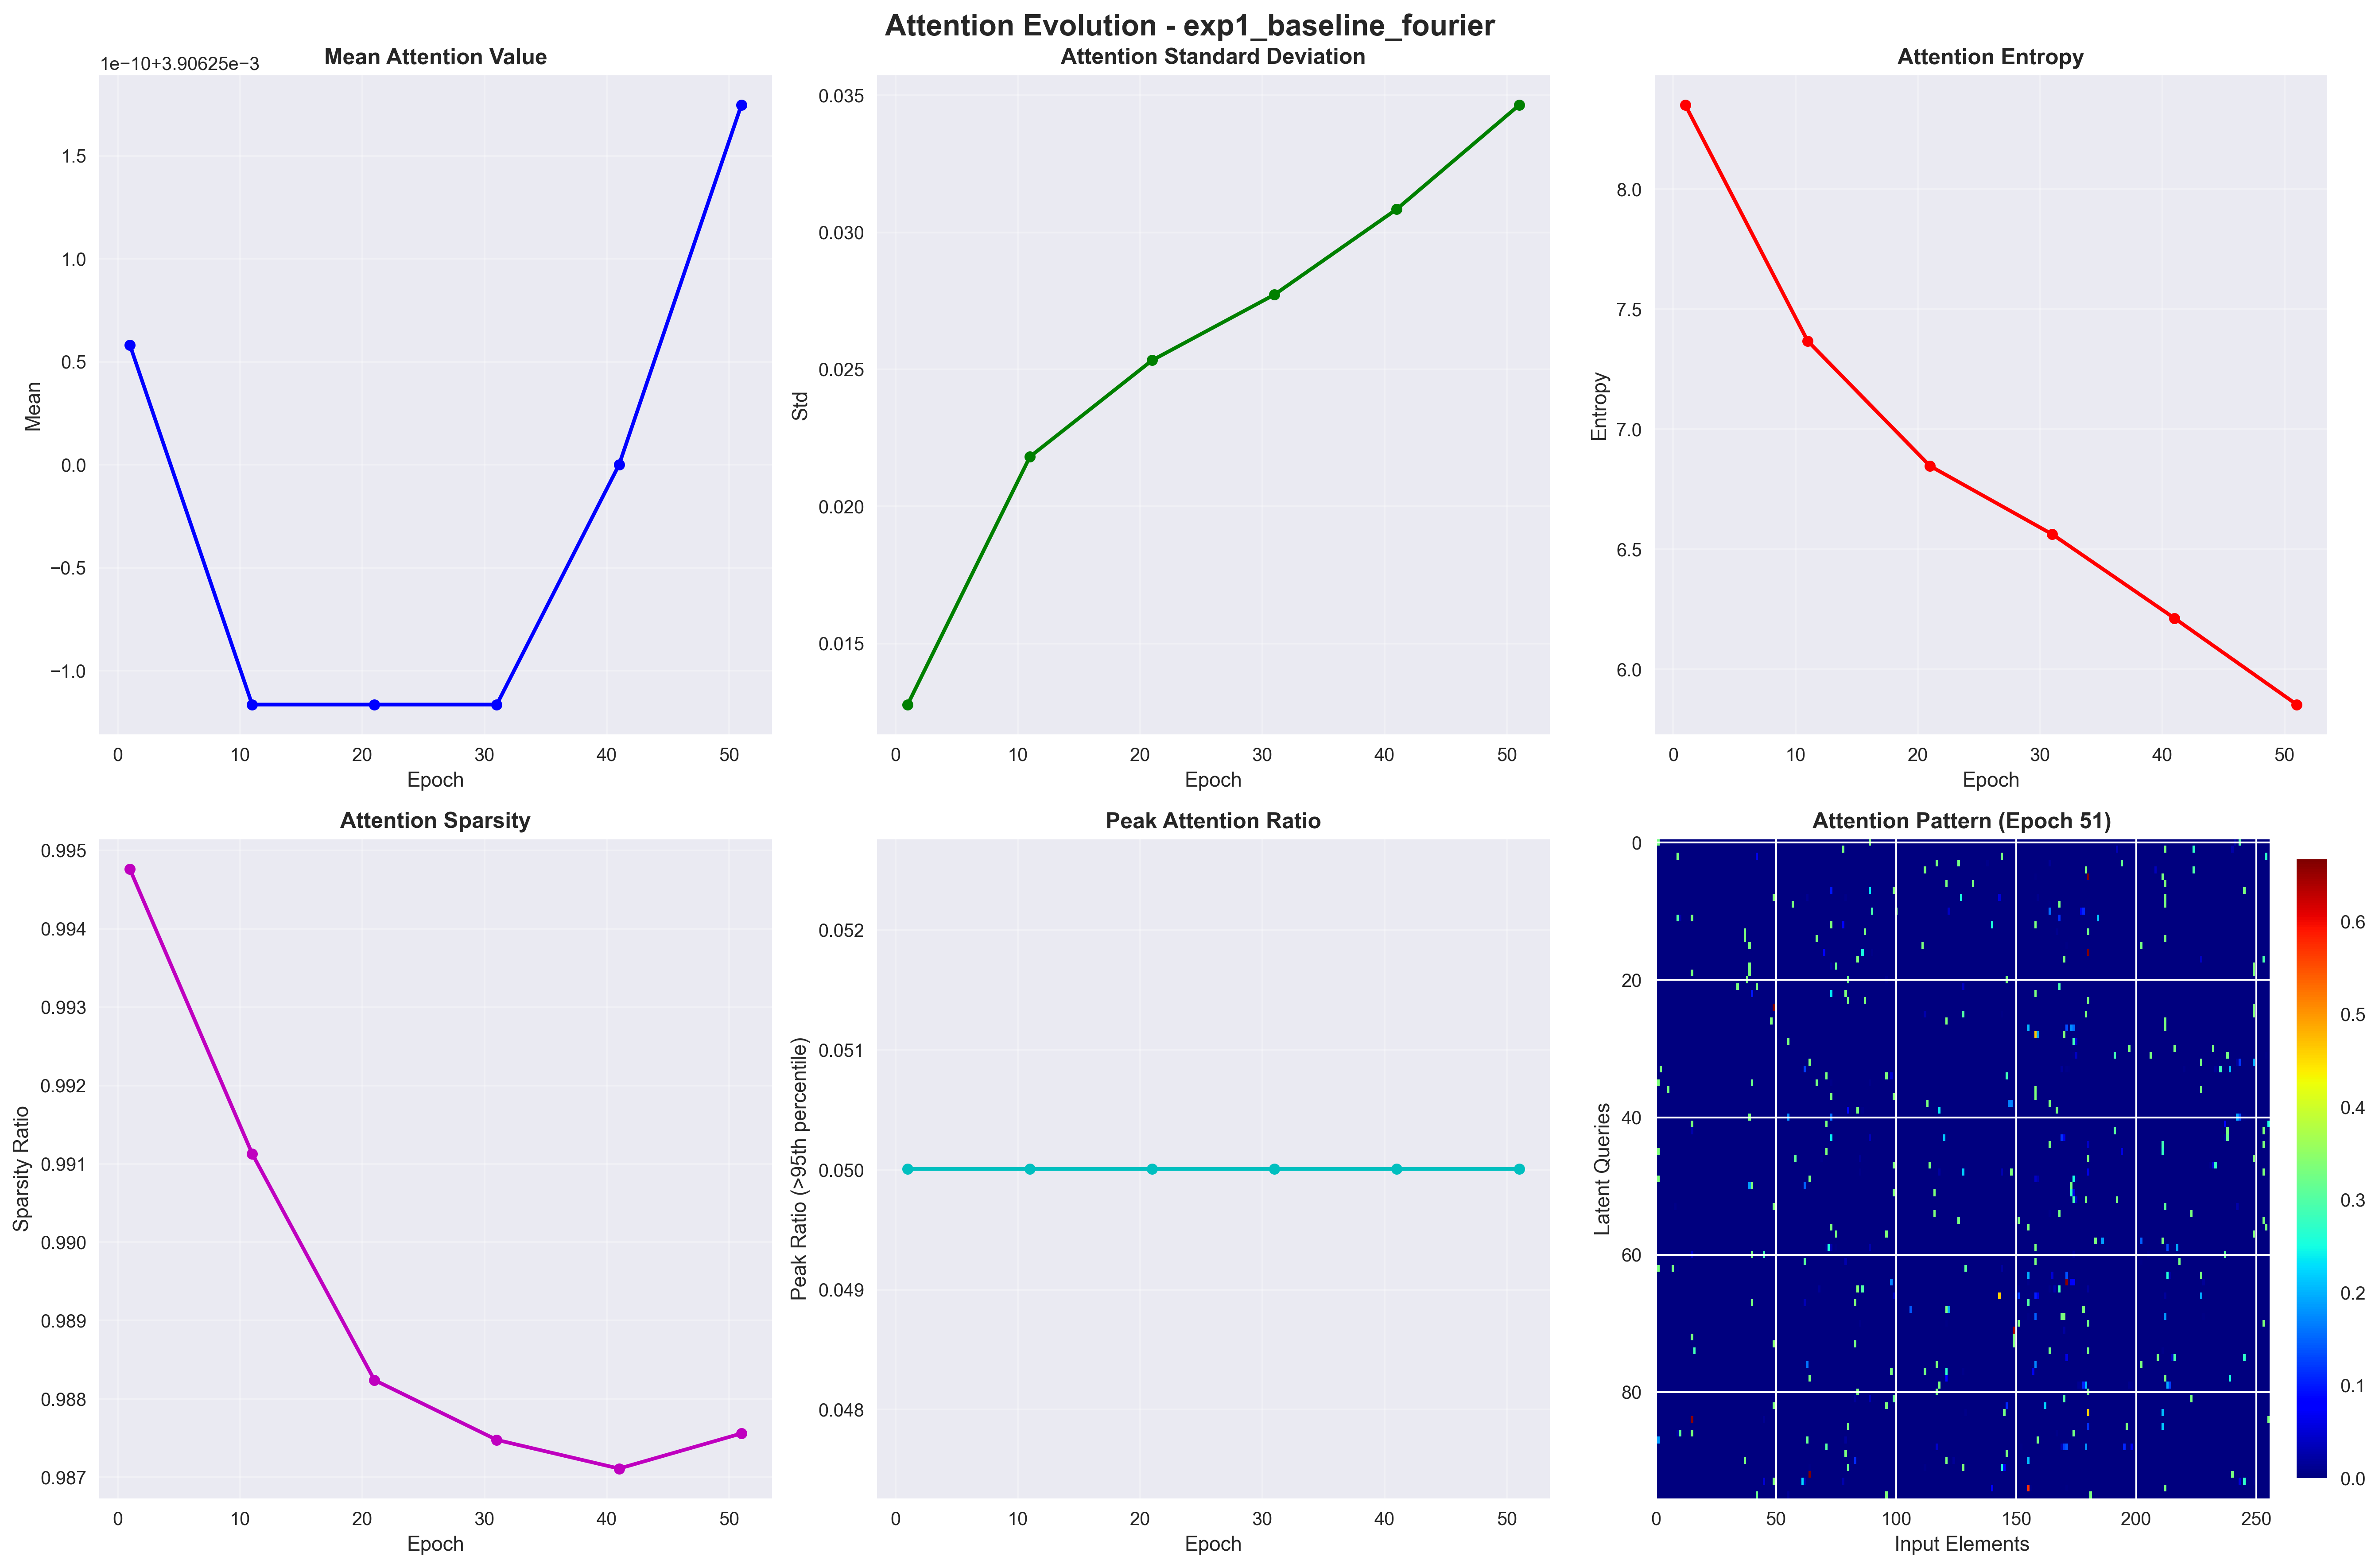
\includegraphics[width=0.9\textwidth,height=0.45\textheight,keepaspectratio]{exp1_baseline_fourier_evolution.png}
      \end{center}

      \vspace{0.2em}
      {\small Structured, spatially selective patterns (entropy $\sim$5.9). Latents specialize in different image regions.}
    \end{column}
    \begin{column}{0.48\textwidth}
      \begin{center}
        \textbf{RGB Only --- no PE (final maps)}\\[2pt]
        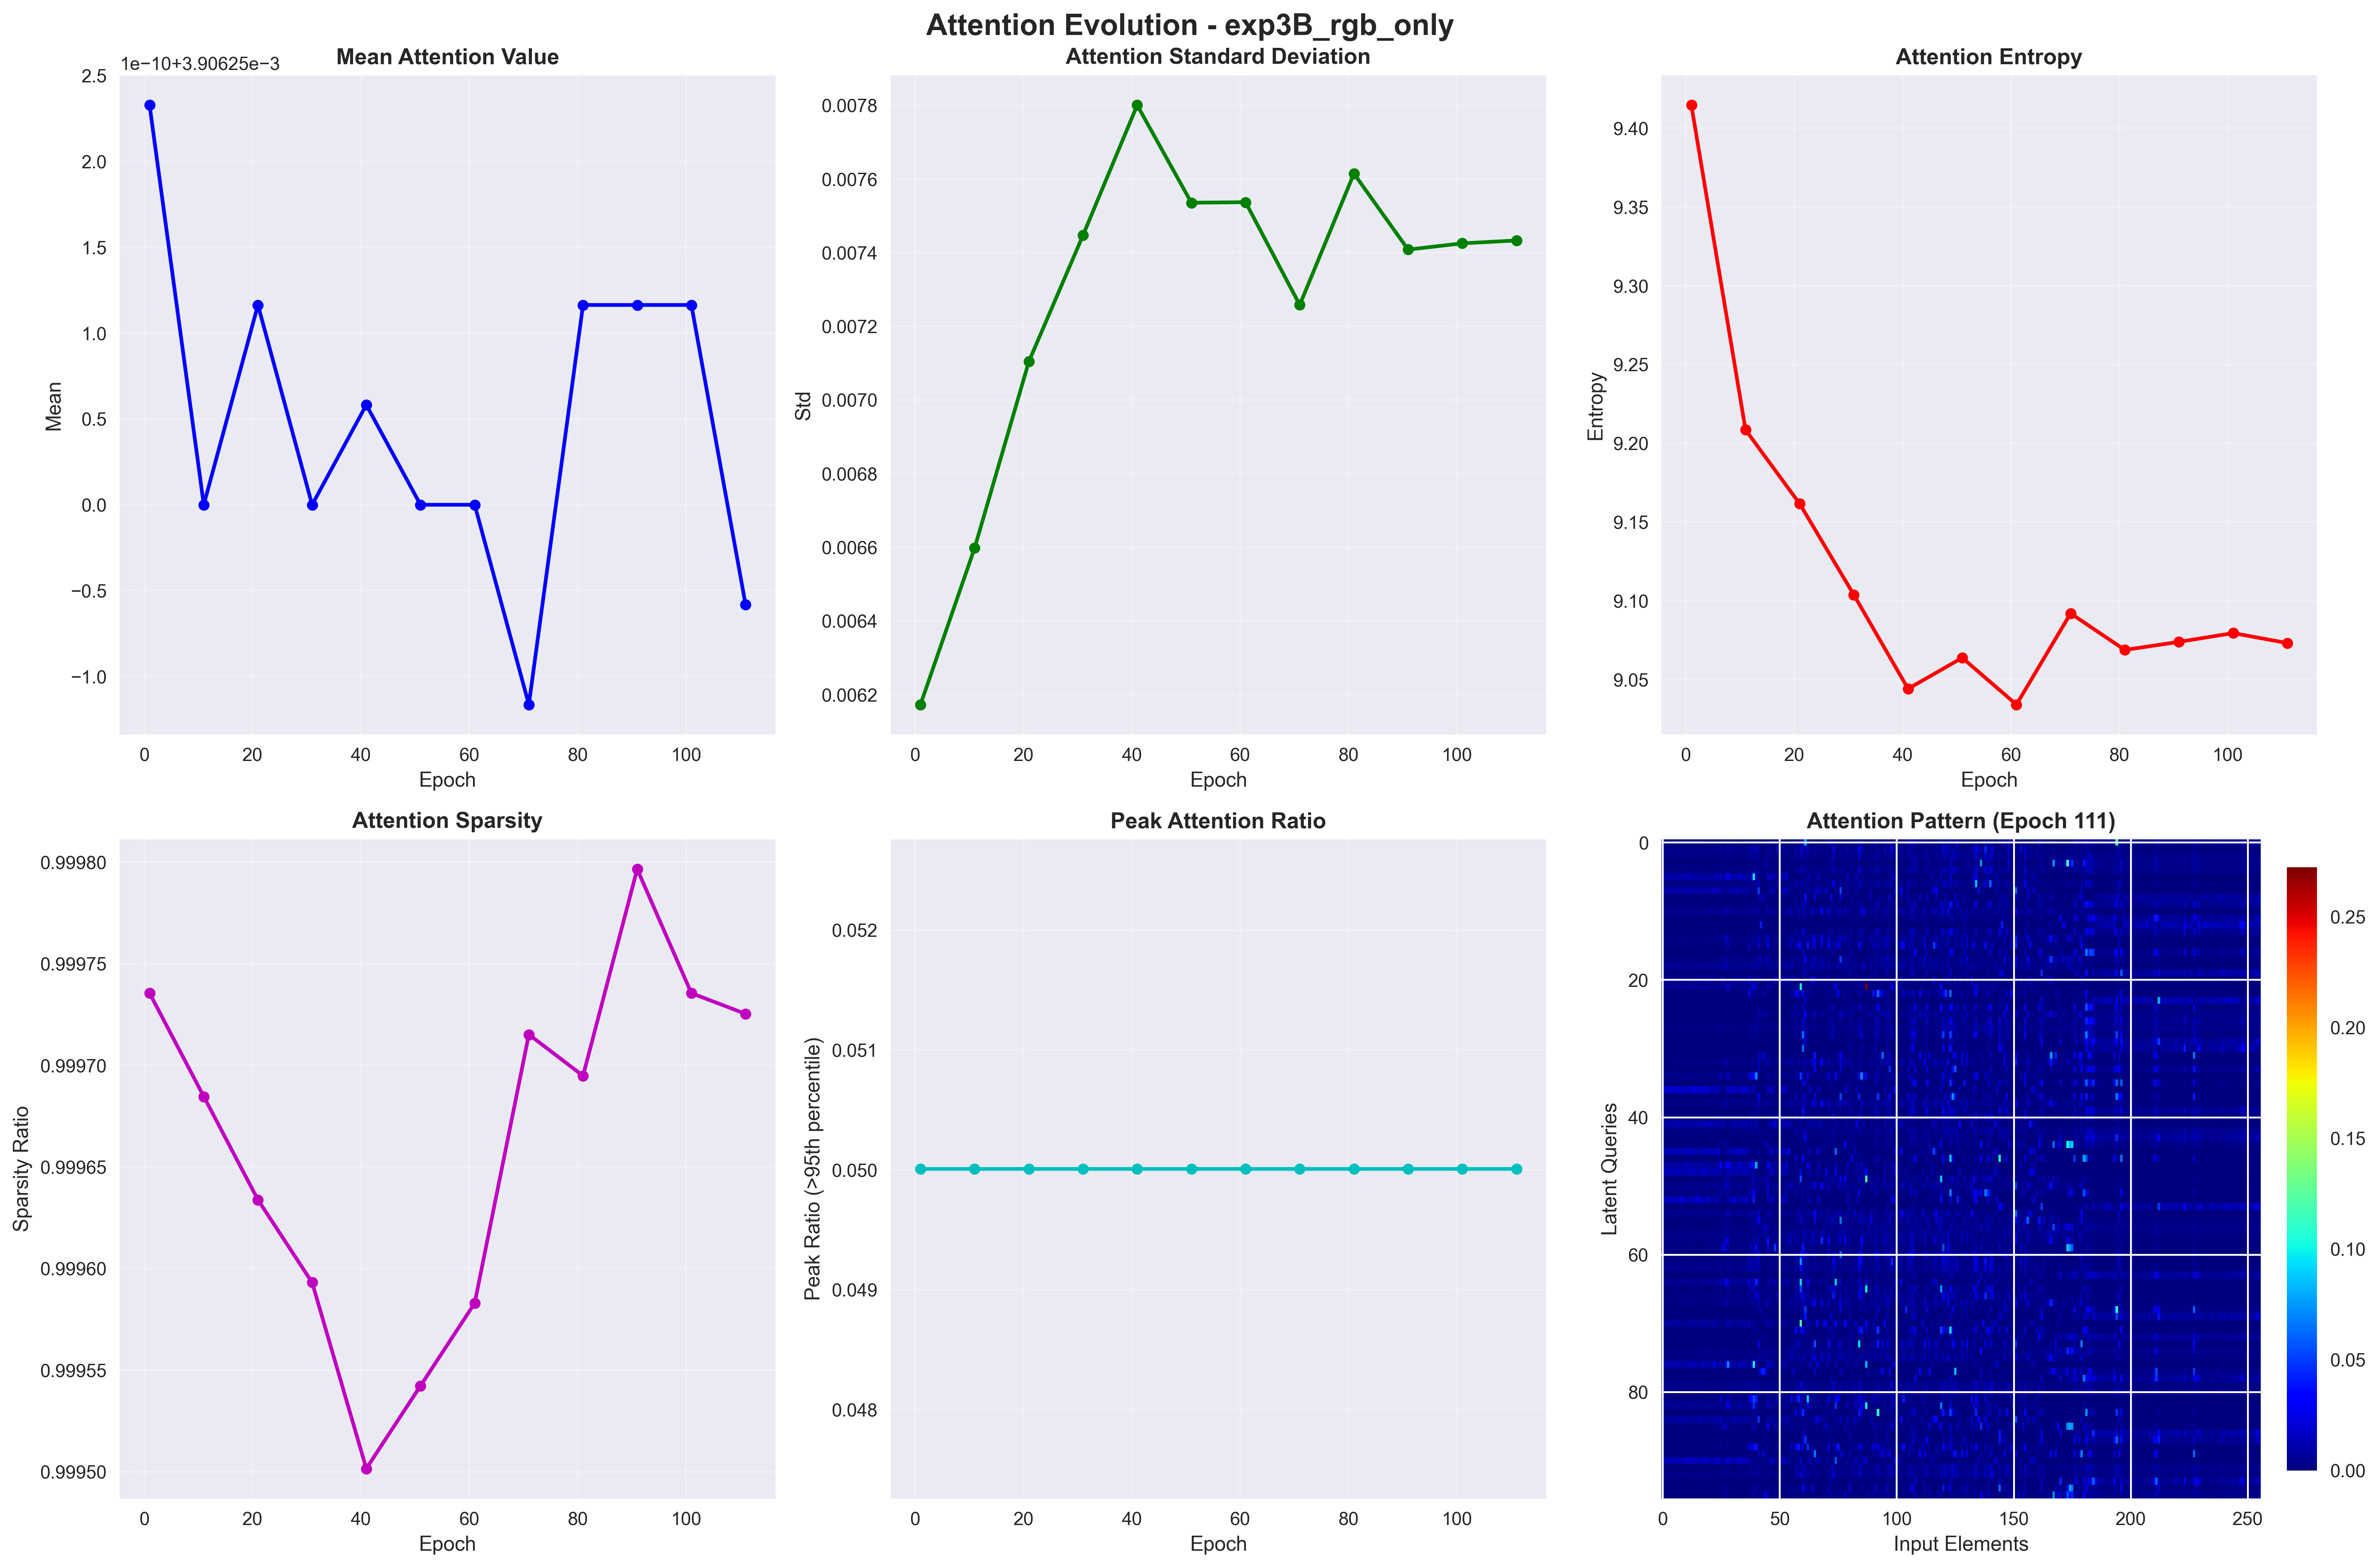
\includegraphics[width=0.9\textwidth,height=0.45\textheight,keepaspectratio]{exp3B_rgb_only_evolution.png}
      \end{center}

      \vspace{0.2em}
      {\small Diffuse, near-uniform patterns (entropy $\sim$9.1). No spatial selectivity --- the model cannot localize information.}
    \end{column}
  \end{columns}

  \vspace{0.3em}
  \begin{block}{Interpretation}
    With Fourier PE, cross-attention learns spatially coherent patterns across training.
    Without PE, attention entropy remains high and patterns lack structure.
  \end{block}
\end{frame}

% ── Slide 28: Comprehensive Results Summary ──────────────────────────────────
\begin{frame}[shrink=5]{Comprehensive Results Summary}
  \begin{table}
    \centering\small
    \begin{tabular}{llccl}
      \toprule
      \textbf{Modality} & \textbf{Model} & \textbf{Best Acc.} & \textbf{Reference} & \textbf{Experiments} \\
      \midrule
      Images (CIFAR-10) & Perceiver & 72.91\% & $>$90\%$^{\dagger}$ & \textbf{23} runs \\
      Images (CIFAR-10) & Perceiver IO & \textcolor{gray}{not run} & --- & 2 pending \\
      Point Clouds (ModelNet40) & Perceiver & \textbf{87.36\%} & 85.7\% & 3 augmentations \\
      Text (WikiText-103) & Perceiver IO & \textbf{86.68\%} MLM & 0.39\% chance & 1 \\
      NLU (GLUE, 8 tasks) & Perceiver IO & \textcolor{gray}{not run} & 81.0 (paper) & 11 pending \\
      \bottomrule
    \end{tabular}
  \end{table}

  {\scriptsize $^{\dagger}$ Strong ViT/CNN baselines on CIFAR-10; neither Perceiver paper benchmarks CIFAR-10, so this column is context, not a target.}

  \vspace{0.4em}
  \begin{columns}[T]
    \begin{column}{0.48\textwidth}
      \textbf{What is measured}
      \begin{itemize}\small
        \item ModelNet40 \textbf{beats} the paper: $+$1.66pp
        \item Best CIFAR-10 run: $T{=}1$, 72.91\%, with 15\% fewer parameters than the baseline
        \item Noise band \textbf{2.78pp}, measured on 3 seed replicas
        \item 11 of 23 CIFAR runs are conclusive
      \end{itemize}
    \end{column}
    \begin{column}{0.48\textwidth}
      \textbf{Scope of the campaign}
      \begin{itemize}\small
        \item Declarative registry of \textbf{42 runs}, \textbf{27} completed
        \item 3 modalities: 2D images, 3D point clouds, raw bytes
        \item One command per run: \texttt{experiments.py --run <id>}
        \item \textbf{15 runs pending}, almost all on the Perceiver IO branch
      \end{itemize}
    \end{column}
  \end{columns}
\end{frame}

% ══════════════════════════════════════════════════════════════════════════════
% SECTION 4: Criticalities & Discussion (slides 29-33)
% ══════════════════════════════════════════════════════════════════════════════
\section{Conclusion}

% ── Slide 29: Gap vs Original Paper ──────────────────────────────────────────
\begin{frame}[shrink=10]{Gap vs Original Papers}
  \begin{columns}[T]
    \begin{column}{0.48\textwidth}
      \textbf{ModelNet40 (Point Clouds):}
      \begin{table}
        \centering\small
        \begin{tabular}{lc}
          \toprule
          \textbf{Source} & \textbf{Acc.} \\
          \midrule
          Original Paper & 85.7\% \\
          This implementation & \textbf{87.36\%} \\
          \midrule
          \textbf{Gap} & \textcolor{AccentGreen}{\textbf{$+$1.66pp}} \\
          \bottomrule
        \end{tabular}
      \end{table}

      \vspace{0.3em}
      \textbf{We are above the paper.}\\
      With a batch $16\times$ smaller (32 vs 512). Plausible because ModelNet40 is small and canonically aligned, so the large-batch advantage counts for little.
    \end{column}
    \begin{column}{0.48\textwidth}
      \textbf{CIFAR-10 (Images):}
      \begin{table}
        \centering\small
        \begin{tabular}{lc}
          \toprule
          \textbf{Source} & \textbf{Acc.} \\
          \midrule
          ViT/CNN baseline & $>$90\% \\
          Best Perceiver run & 72.91\% \\
          \midrule
          \textbf{Gap} & \textcolor{AccentRed}{\textbf{$\sim$17pp}} \\
          \bottomrule
        \end{tabular}
      \end{table}

      \vspace{0.3em}
      \textbf{Larger image gap.}\\
      Reference is strong ViT/CNN baselines --- neither Perceiver paper benchmarks CIFAR-10. Scale gap: TPU cluster vs single GPU, 1\,024 pixels vs 50\,176.
    \end{column}
  \end{columns}

  \vspace{0.5em}
  \begin{block}{Scale factors}
    The CIFAR-10 gap is primarily due to \textbf{batch size} (64 vs 1024), \textbf{latent count} (96 vs 256), and \textbf{compute time} limitations. The Perceiver architecture is particularly sensitive to these scaling factors on image data.
  \end{block}
\end{frame}

% ── Slide 30: Hardware Limitations ───────────────────────────────────────────
\begin{frame}[shrink=8]{Hardware Limitations \& Design Choices}
  \begin{table}
    \centering\small
    \begin{tabular}{lcc}
      \toprule
      \textbf{Parameter} & \textbf{Original Paper (Google)} & \textbf{Project Setup} \\
      \midrule
      Hardware & 512 TPU v3 cores & 1 NVIDIA consumer GPU \\
      Batch size & up to 1024 & max 64--128 \\
      Latents ($N$) & 256--512 & 96--128 \\
      Model size & 30--100M+ params & 3.35--10M params \\
      Training time & days (distributed) & hours--days (single GPU) \\
      \bottomrule
    \end{tabular}
  \end{table}

  \vspace{0.5em}
  \begin{columns}[T]
    \begin{column}{0.48\textwidth}
      \textbf{Consequences:}
      \begin{itemize}
        \item LAMB optimizer less effective with small batches
        \item Fewer latents limit representational capacity
        \item Reduced augmentation due to time constraints
        \item Fewer hyperparameter search iterations
      \end{itemize}
    \end{column}
    \begin{column}{0.48\textwidth}
      \textbf{Mitigation strategies:}
      \begin{itemize}
        \item Weight sharing to reduce memory
        \item Gradient accumulation where possible
        \item Careful cosine annealing schedule
        \item Focus experiments on most informative ablations
      \end{itemize}
    \end{column}
  \end{columns}
\end{frame}

% ── Slide 31: Possible Improvements ──────────────────────────────────────────
\begin{frame}[shrink=9]{Possible Improvements}
  \begin{columns}[T]
    \begin{column}{0.48\textwidth}
      \textbf{Architecture:}
      \begin{itemize}
        \item Increase latent count ($N = 256$+) with gradient checkpointing
        \item Add multi-scale cross-attention (coarse $\rightarrow$ fine)
        \item Explore relative positional encodings (RoPE, ALiBi)
        \item Deeper decoder for structured outputs
      \end{itemize}

      \vspace{0.5em}
      \textbf{Training:}
      \begin{itemize}
        \item Larger batch sizes with gradient accumulation
        \item Mixed precision (FP16/BF16) training
        \item Longer training schedules
        \item Advanced augmentation (CutMix, MixUp)
      \end{itemize}
    \end{column}
    \begin{column}{0.48\textwidth}
      \textbf{Data \& Tasks:}
      \begin{itemize}
        \item ImageNet pre-training for vision
        \item Subword tokenization for NLP
        \item Multi-modal joint training
        \item Audio modality experiments
      \end{itemize}

      \vspace{0.5em}
      \textbf{Analysis:}
      \begin{itemize}
        \item Layer-wise attention probing
        \item Latent space clustering visualization
        \item Systematic hyperparameter search
        \item Comparison with efficient Transformers (Linformer, Performer)
      \end{itemize}
    \end{column}
  \end{columns}
\end{frame}

% ── Slide 32: Lessons Learned ────────────────────────────────────────────────
\begin{frame}[shrink=5]{Empirical Summary}
  \begin{columns}[T]
    \begin{column}{0.48\textwidth}
      \textbf{Conclusive (outside the 2.78pp band):}
      \begin{itemize}\small
        \item \textbf{Generality}: one architecture, 87.36\% on 3D point clouds --- above the paper --- and 86.68\% on raw bytes
        \item \textbf{Where} capacity goes beats \textbf{how much}: 6.1M$\to$12.2M$\to$18.3M params gives 68.98$\to$67.24$\to$67.05\%
        \item \textbf{Latent init scale} is the critical hyperparameter: 0.02$\to$71.63\%, 1.0$\to$52.08\%
        \item \textbf{Interleaving} cross-attends beats front-loading by 4.44pp
        \item \textbf{Rotation augmentation} costs 13.29pp on ModelNet40
      \end{itemize}
    \end{column}
    \begin{column}{0.48\textwidth}
      \textbf{Inside the band --- ``no measurable damage'':}
      \begin{itemize}\small
        \item Permutation invariance, with \emph{both} positional encodings
        \item Weight sharing: $3.1\times$ fewer parameters at no measurable cost
        \item Fourier vs learned PE at this scale
      \end{itemize}

      \vspace{0.4em}
      \textbf{Not measured --- runs still pending:}
      \begin{itemize}\small
        \item Lower bound with no positional encoding
        \item Perceiver vs Perceiver IO on images
        \item The GLUE average (0 of 8 tasks)
        \item A convolutional baseline
      \end{itemize}
    \end{column}
  \end{columns}

  \vspace{0.5em}
  \begin{block}{Central methodological finding}
    Measuring the \textbf{noise band} --- three replicas differing only by seed --- cost two runs and changed the status of all the others. Without it, 9 of the 23 comparisons would have been reported as effects when they are variance.
  \end{block}
\end{frame}

% ── Slide 33: Conclusions ────────────────────────────────────────────────────
\begin{frame}[shrink=15]{Conclusions}
  \begin{columns}[T]
    \begin{column}{0.48\textwidth}
      \textbf{Architecture properties:}
      \begin{itemize}
        \item Single architecture for images, point clouds, and text
        \item Linear complexity in input size
        \item Memory efficiency via weight sharing ($\sim$61\%)
        \item Zero CNN/RNN domain-specific assumptions
        \item Output queries enable flexible structured decoding
      \end{itemize}
    \end{column}
    \begin{column}{0.48\textwidth}
      \textbf{Remaining limitations:}
      \begin{itemize}
        \item Requires large compute to match specialized models
        \item Heavily depends on positional encoding
        \item Outperformed by efficient CNNs on standard vision benchmarks
        \item LAMB optimizer introduces training instability at small scale
        \item Latent bottleneck limits fine-grained spatial reasoning
      \end{itemize}
    \end{column}
  \end{columns}

  \vspace{0.5em}
  \begin{exampleblock}{Closing statement}
    The experiments show that a \textbf{single general-purpose architecture} can be applied to images, point clouds, and text. At the tested scale, performance depends strongly on positional encoding, latent capacity, and available training compute.
  \end{exampleblock}
\end{frame}

% ══════════════════════════════════════════════════════════════════════════════
% SECTION 5: Closing (slides 34-36)
% ══════════════════════════════════════════════════════════════════════════════
% Closing materials: references and appendix.

% ── Slide 35: Appendix – Expected Questions ──────────────────────────────────
% (References and Expected-Questions slides removed)

% ── Slide 36: Thank You ──────────────────────────────────────────────────────
\begin{frame}
  \begin{center}
    {\Huge\color{UnifiBlue}\textbf{Thank you!}}\\[1.5em]
    {\Large\color{UnifiDark} Questions?}\\[2.5em]
    {\color{UnifiDark}Francesco Gigli and Corso Vignoli}\\[0.3em]
    {\small\color{UnifiDark} Code and models available upon request}
  \end{center}
\end{frame}

\end{document}
